\documentclass[11pt,]{article}
\usepackage{lmodern}
\usepackage{amssymb,amsmath}
\usepackage{ifxetex,ifluatex}
\usepackage{fixltx2e} % provides \textsubscript
\ifnum 0\ifxetex 1\fi\ifluatex 1\fi=0 % if pdftex
  \usepackage[T1]{fontenc}
  \usepackage[utf8]{inputenc}
\else % if luatex or xelatex
  \ifxetex
    \usepackage{mathspec}
    \usepackage{xltxtra,xunicode}
  \else
    \usepackage{fontspec}
  \fi
  \defaultfontfeatures{Mapping=tex-text,Scale=MatchLowercase}
  \newcommand{\euro}{€}
    \setmainfont{Georgia}
\fi
% use upquote if available, for straight quotes in verbatim environments
\IfFileExists{upquote.sty}{\usepackage{upquote}}{}
% use microtype if available
\IfFileExists{microtype.sty}{%
\usepackage{microtype}
\UseMicrotypeSet[protrusion]{basicmath} % disable protrusion for tt fonts
}{}
\usepackage[margin=0.5in]{geometry}
\usepackage{color}
\usepackage{fancyvrb}
\newcommand{\VerbBar}{|}
\newcommand{\VERB}{\Verb[commandchars=\\\{\}]}
\DefineVerbatimEnvironment{Highlighting}{Verbatim}{commandchars=\\\{\}}
% Add ',fontsize=\small' for more characters per line
\usepackage{framed}
\definecolor{shadecolor}{RGB}{248,248,248}
\newenvironment{Shaded}{\begin{snugshade}}{\end{snugshade}}
\newcommand{\KeywordTok}[1]{\textcolor[rgb]{0.13,0.29,0.53}{\textbf{{#1}}}}
\newcommand{\DataTypeTok}[1]{\textcolor[rgb]{0.13,0.29,0.53}{{#1}}}
\newcommand{\DecValTok}[1]{\textcolor[rgb]{0.00,0.00,0.81}{{#1}}}
\newcommand{\BaseNTok}[1]{\textcolor[rgb]{0.00,0.00,0.81}{{#1}}}
\newcommand{\FloatTok}[1]{\textcolor[rgb]{0.00,0.00,0.81}{{#1}}}
\newcommand{\CharTok}[1]{\textcolor[rgb]{0.31,0.60,0.02}{{#1}}}
\newcommand{\StringTok}[1]{\textcolor[rgb]{0.31,0.60,0.02}{{#1}}}
\newcommand{\CommentTok}[1]{\textcolor[rgb]{0.56,0.35,0.01}{\textit{{#1}}}}
\newcommand{\OtherTok}[1]{\textcolor[rgb]{0.56,0.35,0.01}{{#1}}}
\newcommand{\AlertTok}[1]{\textcolor[rgb]{0.94,0.16,0.16}{{#1}}}
\newcommand{\FunctionTok}[1]{\textcolor[rgb]{0.00,0.00,0.00}{{#1}}}
\newcommand{\RegionMarkerTok}[1]{{#1}}
\newcommand{\ErrorTok}[1]{\textbf{{#1}}}
\newcommand{\NormalTok}[1]{{#1}}
\usepackage{graphicx}
\makeatletter
\def\maxwidth{\ifdim\Gin@nat@width>\linewidth\linewidth\else\Gin@nat@width\fi}
\def\maxheight{\ifdim\Gin@nat@height>\textheight\textheight\else\Gin@nat@height\fi}
\makeatother
% Scale images if necessary, so that they will not overflow the page
% margins by default, and it is still possible to overwrite the defaults
% using explicit options in \includegraphics[width, height, ...]{}
\setkeys{Gin}{width=\maxwidth,height=\maxheight,keepaspectratio}
\ifxetex
  \usepackage[setpagesize=false, % page size defined by xetex
              unicode=false, % unicode breaks when used with xetex
              xetex]{hyperref}
\else
  \usepackage[unicode=true]{hyperref}
\fi
\hypersetup{breaklinks=true,
            bookmarks=true,
            pdfauthor={},
            pdftitle={},
            colorlinks=true,
            citecolor=blue,
            urlcolor=blue,
            linkcolor=magenta,
            pdfborder={0 0 0}}
\urlstyle{same}  % don't use monospace font for urls
\setlength{\parindent}{0pt}
\setlength{\parskip}{6pt plus 2pt minus 1pt}
\setlength{\emergencystretch}{3em}  % prevent overfull lines
\setcounter{secnumdepth}{0}

%%% Use protect on footnotes to avoid problems with footnotes in titles
\let\rmarkdownfootnote\footnote%
\def\footnote{\protect\rmarkdownfootnote}

%%% Change title format to be more compact
\usepackage{titling}

% Create subtitle command for use in maketitle
\newcommand{\subtitle}[1]{
  \posttitle{
    \begin{center}\large#1\end{center}
    }
}

\setlength{\droptitle}{-2em}
  \title{}
  \pretitle{\vspace{\droptitle}}
  \posttitle{}
  \author{}
  \preauthor{}\postauthor{}
  \date{}
  \predate{}\postdate{}

\usepackage{booktabs}
\usepackage[font={small},labelfont=bf,labelsep=colon]{caption}
\linespread{0.9}
\usepackage[compact]{titlesec}
\usepackage{enumitem}
\usepackage{tikz}
\def\checkmark{\tikz\fill[scale=0.4](0,.35) -- (.25,0) -- (1,.7) -- (.25,.15) -- cycle;}
\setlist{nolistsep}
\titlespacing{\section}{2pt}{*0}{*0}
\titlespacing{\subsection}{2pt}{*0}{*0}
\titlespacing{\subsubsection}{2pt}{*0}{*0}
\setlength{\parskip}{3pt}
\setlength{\topsep}{0pt}
\setlength{\partopsep}{0pt}
\setlength{\itemsep}{0pt}
\setlength{\floatsep}{0pt}
\setlength{\intextsep}{2pt}
\setlength{\abovecaptionskip}{2pt}
\setlength{\belowcaptionskip}{0pt}


\begin{document}

\maketitle


\pagenumbering{gobble}

\begin{center}
{\Large \bf ITK-Lung:  A Software Framework for Lung Image Processing and Analysis}
\end{center}

\section{2 Specific Aims}\label{specific-aims}

The development and proliferation of quantitative image analysis methods
have accelerated research efforts and are having an increasingly
significant impact in modern clinical practice. Although the research
utility of these techniques has been amply demonstrated in determining
longitudinal and groupwise trends, they are also becoming increasingly
relevant in the clinical setting in providing biomarkers for aiding
patient diagnoses, monitoring disease progression, and determining
treatment outcomes. Increases in the capabilities and accessibility of
computational facilities and a corresponding sophistication in
computational algorithms have only made such practices more commonplace.

One of the most significant hurdles in adopting more quantitative
clinical practices and exploring additional novel research pathways is
the availability of accurate, robust, and easy-to-use image analysis
tools. Historically, the research and clinical communities (and their
overlap) have significantly benefited from computational image analysis
packages, particularly those softwares which have been tailored for
specific application domains. Although several such established packages
exist for neuroimaging research (e.g., FSL, FreeSurfer, AFNI, SPM),
\emph{no such package exists for pulmonary imaging analysis. The primary
goal of this project is to develop a robust, open-source image analysis
toolkit and dissemination platform specifically targeted at the
pulmonary research community.}

Although methodological research is continually being presented at
conferences and published in various venues, the unfortunate reality is
that much of this work exists strictly in ``advertisement'' form.
Oftentimes the underlying code is unavailable to other researchers or is
implemented in a limited manner (i.e., strictly as proof-of-concept
software). Frequently, crucial parameter choices are omitted in the
corresponding publication(s) which makes external implementations
difficult. In addition, the data used to showcase the proposed
methodologies are often private and actual data visualization is limited
to carefully selected snapshots for publication purposes which might not
be representative of algorithmic performance. Finally, many of these
analysis methods are patented and/or integrated into proprietary
commercial software packages which severely limits accessibility to
researchers.

As a corrective alternative, this project brings together leading
expertise in lung imaging research at Penn and UVa to develop, evaluate
and deploy under community support an open-source software toolkit
targeted for pulmonary imaging research. As principal developers of the
popular, open-source ANTs, ITK-SNAP and ITK packages, we have extensive
experience in the development of well-written software that has gained
much traction in the neuroscience community and propose to leverage and
enhance these advanced packages to make a similar impact in the
pulmonary community with this project. Specifically, we plan to provide
methods for core pulmonary image analysis tasks across multiple
modalities, many of which we have proposed in past work. These basic
tasks include pulmonary image registration, template building for
cross-sectional and longitudinal (i.e., respiratory cycle) analyses,
functional and structural lung image segmentation, and computation of
quantitative image indices as potential imaging biomarkers. In addition
to the software, we will provide scripts, documentation, and tutorial
materials consistent with open-science principles. Formally, this
project is defined by the following specific aims:

\begin{itemize}
\itemsep1pt\parskip0pt\parsep0pt
\item
  \textbf{Specific Aim 1:} \textbf{Develop ITK-Lung, a set of
  open-source software tools for CT, proton, and He-3 pulmonary
  computational analysis.} These open-source software tools will
  specifically target pulmonary image analysis and comprise core
  application functions such as inspiratory/expiratory registration,
  ventilation-based segmentation, lung and lobe estimation, airway and
  vessel segmentation, nodule detection, and calculation of clinical
  indices for characterization of lung development and pathology. To
  support these software development efforts, CT and 1H MRI multi-atlas
  libraries will be provided as open data complete with the
  corresponding lung, airway, vessel, and lobe segmentations according
  to modality. In addition, we will generate optimal intensity/shape
  templates from each library. Both sets of data will be provided with
  the scripts used to produce them in order to permit user-reproduction
  of the results. As developers of several leading open-source
  applications for image segmentation and registration, we know
  firsthand that the impact of a particular technological innovation
  greatly depends on the availability of an easily accessible software
  implementation. The proposed software framework will tie together all
  of the capabilities of the project's developed methodology in the form
  of programmable workflows and provide a seamless user experience
  through a full featured graphical user interface. Interactive
  functionality will extend beyond the ability to steer segmentation and
  registration pipelines to include tools for evaluation and
  visualization of processed results.
\item
  \textbf{Specific Aim 2:} \textbf{Validate and disseminate the
  developed ITK-Lung resources by leveraging use cases from a broad
  network of partner investigators representing the state-of-the-science
  in lung imaging research.} This aim will evaluate and refine the
  developed methodology within the real-world context of pulmonary
  research being carried out at various partner sites. We will
  disseminate the results of the project through open-source
  distribution of the software, atlases and documentation, online user
  support, and conduct of hands-on training workshops.
\end{itemize}

\newpage

\section{3 Research Strategy}\label{research-strategy}

\subsection{\textbf{3(a) Significance}}\label{a-significance}

\textbf{3(a.1) The importance of pulmonary image analysis tools for
research and clinical investigation.} The increased utilization of
imaging for both research and clinical purposes has furthered the demand
for quantitative image analysis techniques. The use of these
computational techniques is motivated by the need for less subjectivity
and more standardization in medical image interpretation, increased
speed and automation in diagnosis, and greater robustness and accuracy
for determining biological correlates with imaging findings. For
example, in the area of pharmaceutical development and testing, imaging
biomarkers are crucial. In order to determine fundamental study
parameters such as drug safety and effectiveness, quantitative
assessments derived from imaging measures must be objective and
reproducible {[}1{]} which is often difficult without computational aid
given the intra- and inter-reader variability in radiological practice
{[}2, 3{]}. Additionally, the exciting possibilities associated with
``big data'' and the potential for improvement in individualized,
evidence-based medicine has also increased the need for sophisticated
data transformation and machine learning techniques.

\textbf{3(a.2) Open-source as an essential attribute of high-impact
image analysis toolkits.} Well-vetted and publicly available software is
a significant benefit to targeted research communities. For example, the
neuroscience community has greatly benefited from highly evolved
software packages such as FreeSurfer {[}4{]}, the FMRIB Software Library
(FSL) {[}5{]}, the Analysis of Functional NeuroImages (AFNI) package
{[}6{]}, the Statistical Parametric Mapping (SPM) package {[}7{]}, and
several others. Performing a pubmed query for any one of these softwares
every year for the past decade (cf Figure 1) illustrates the growing use
of such packages and the research studies that are produced as a result.
However, despite the absolute number of articles produced using such
software and the year-by-year usage increase, no such analogous set of
tools exist for pulmonary-specific research. In fact, in a recent review
of CT- and MRI-derived biomarkers for pulmonary clinical investigation,
the authorial consensus is that ``{[}the absence of{]} universally
available image analysis software'' is a major hinderance to more
widespread usage of such imaging biomarkers {[}8{]}.

\begin{figure}[htbp]
\centering
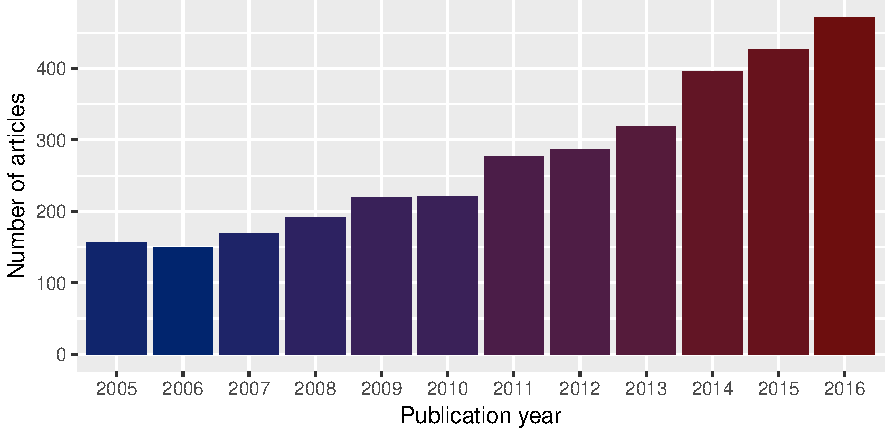
\includegraphics{stitched_files/figure-latex/pubmedQuery-1.pdf}
\caption{Number of articles per year which cite publicly available
neuroimaging analysis packages (specifically, FreeSurfer, AFNI, FSL, and
SPM). Although the benefits seem clear for the neuroscience community,
analogous efforts within the pulmonary community have yet to be
undertaken despite consensus amongst researchers and clinicians
regarding the utility of such offerings.}
\end{figure}

Medical image analysis libraries (e.g., the NIH-sponsored Insight
ToolKit) provide extensive algorithmic capabilities for a range of
generic image processing tasks. However, tailored software packages for
certain application domains (e.g., lung image analysis) are not
available despite the vast number of algorithms that have been proposed
in the literature. It is important to note that the goals of this
project would significantly support the National Library of Medicine's
own open-source directives in that all software would be developed using
the established Insight ToolKit's coding and testing standards with the
specific objective that all project code would be contributed for
inclusion in future versions of the Insight ToolKit as we have done in
the past. It should also be noted that open-source software, in general,
has documented benefits within the targeted communities for which it is
developed and supported. In addition to the increase in research output
illustrated earlier, open-source permits students and researchers to
learn specific computational techniques in a social environment {[}9{]}.
This, in turn, provides motivation for user-based support including
potential contributions such as bug fixes and feature additions.
Additional analyses have shown the tremendous cost savings that
open-source software yields {[}10{]}. Furthermore, open-source
development and distribution within a large, and well-invested community
(such as ITK) takes advantage of Linus's law, i.e., ``given enough
eyeballs, all bugs are shallow," for producing robust software.

\subsection{\textbf{3(b) Innovation}}\label{b-innovation}

\textbf{3(b.1) Open-source pulmonary imaging algorithmic innovation.}
Given the lack of open-source solutions for pulmonary image analysis,
this project would produce the first-of-its-kind processing and analytic
platform for performing such research. Similar to the brain-specific
algorithms provided in our ANTs toolkit, our project would include the
most essential algorithms for analyzing lung images from different
modalities including CT, 3He, and 1H MRI. \emph{Many algorithms have
been proposed in various technical venues but that which we propose
would provide well-vetted and easy-to-use implementations of specific
robust methodologies for pulmonary medical image analysis, many of which
have been developed by our group.} To facilitate the usage of these
algorithms, we will provide documentation including self-contained
online examples, tutorials, and hands-on training workshops.

\textbf{3(b.2) Use case studies with leading pulmonary research
scientists.} An additional innovative component of the project is the
inclusion of extensive use cases from leading pulmonary imaging research
scientists in various locations with different image acquisition
protocols, equipment, etc. to ensure quality and robustness of the
processed data. Additionally, such use cases involving other groups
would highlight existing deficiencies in algorithmic functionality in
our project which would then be remedied by additional development
efforts. These real-world use cases were solicited representing as
broadly as possible the requirements of the community as well as the
multiple modality and algorithmic variations which commonly occur.

We have partnered with leading pulmonary research groups who are
familiar with our work and who will provide study-specific imaging data
of various modalities which we will then process using the proposed
toolkit. These processed data will be returned to the corresponding
providers with detailed instructions on reproducing these results in
their own labs. Software and tutorial materials drawn from these
experiences will be provided to the public for any interested researcher
to apply to their own data. Given the different image acquisition
sources, this strategy should also demonstrate the robustness of our
tools.

In addition to these collaborative efforts, our own analyses at Penn and
UVa will also be included. Any clinical findings of interest will be
published in traditional venues (e.g., Chest). In addition, we will
provide all the quantitative analysis scripts as a companion release for
the paper (e.g., see previous similar offerings from our group {[}11,
12{]}). Such a comprehensive clinical research investigation using these
tools will not only provide insight into the specifics of certain
pulmonary pathologies but will also offer a reproducible mechanism for
using the tools created in this project.

\subsection{\textbf{3(c) Research design}}\label{c-research-design}

\subsubsection{3(c.1) Preliminary data}\label{c.1-preliminary-data}

\textbf{3(c.1.1) Generic ANTs core tools for image analysis and
processing.} The Advanced Normalization Tools (ANTs) package is a
state-of-the-art, open-source software toolkit for image registration,
segmentation, and other core medical image analysis functionality
{[}13{]}. Several core programs comprising portions of the proposed
pulmonary software framework have been created and made available within
ANTs (and either simultaneously or subsequently made available in ITK).
However, as mentioned earlier, these programs have more general
application and require pulmonary-specific tuning for the tasks targeted
by this project. The following list comprises several core software
tools for tuning, subsequent extensions, documentation, tutorial
generation, and the creation of easy-to-use bash scripts for large-scale
processing of pulmonary imaging data.

\textbf{ANTs image registration.} One of the most important
methodological developments in medical image analysis is the advent of
image registration techniques capable of accommodating the highly
complex inter-individual variations seen in human anatomy. Our team is
well-recognized for seminal contributions to the field that date back to
the original elastic matching method of Bajcsy and co-investigators
{[}14--16{]}. Our most recent work, embodied in the ANTs open-source,
cross-platform toolkit for multiple modality image processing, continues
to set the standard in the field. ANTs not only encodes the most
advanced results in registration research, notably the Symmetric
Normalization (SyN) algorithm for diffeomorphisms {[}17{]}, but also
packages these within a full featured platform that includes an
extensive library of similarity measures, transformation types, and
regularizers. Recently, a thorough comparison with the original SyN
algorithm was performed using a B-spline variant {[}11{]}. This
evaluation utilized multiple publicly available, annotated brain data
sets and demonstrated statistically significant improvement in label
overlap measures. As part of that study, we produced the scripts
\texttt{antsRegistrationSyN.sh} and \texttt{antsRegistrationSyNQuick.sh}
which provide a simple interface to our normalization tools for
brain-specific normalization and are two of the most widely used scripts
in the ANTs toolkit. \emph{Similar to the developments that we are
proposing, these scripts were extensively modified to serve as a
follow-up entry into the EMPIRE10 lung registration challenge where
B-spline SyN performed better than its original counterpart on pulmonary
data {[}18{]}.}

\textbf{Multi-modal template generation.} Given the variability in
anatomical shape across populations and the lack of publicly available
atlases for specific organs, generating population- or subject-specific
optimal shape/intensity templates significantly enhances study potential
{[}19, 20{]}. First, an average template is estimated via a voxel-wise
mean of all the individual subject images. This estimate is iteratively
updated by registering each image to the current template, performing a
voxelwise average to create a new estimate, and then ``reshaping'' this
template based on the average inverse transformation which ``moves'' the
template estimate closer to the group mean---see Figure 2 for a
cohort-specific multi-modal brain template for females in the age range
50--60. This functionality has proven to be a vital component of the
ANTs toolkit for performing neuroimaging research (e.g., {[}12,
21--25{]}). \emph{Similarly, this functionality has also demonstrated
significant importance in pulmonary studies {[}26{]}.}

\textbf{Bayesian segmentation with spatial and MRF priors.} Early
statistically-based segmentation work appropriated NASA satellite image
processing software for classification of head tissues in 2-D MR images
{[}27{]}. Following this work, many researchers adopted statistical
methods for $n$-tissue anatomical brain segmentation. The
Expectation-Maximization (EM) framework is natural {[}28{]} given the
``missing data'' aspect of this problem. Core components of this type of
work include the explicit modeling of the tissue intensity values as
statistical distributions {[}29, 30{]} and the use of Markov Random
Field (MRF) modeling {[}31{]} for regularizing the classification
results {[}32{]}. Spatial prior probability maps of anatomical
structures of interest are also employed within this framework {[}33,
34{]}. Although this particular segmentation framework has significant
application in the neuroimaging domain, it is also relevant to other
domains including functional ventilation of the lung {[}35{]}.
\emph{However, despite the numerous developments which have been
proposed over the years within this area, there are an extremely limited
number of actual software implementations. This deficit inspired us to
create our own Bayesian segmentation framework {[}36{]} (denoted as
Atropos) which we have made publicly available within ANTs and has
proven highly effective in quantification of functional lung imaging
{[}35, 37--39{]}.}

\textbf{N4 bias correction.} Critical to quantitative processing of MRI
is the minimization of field inhomogeneity effects which produce
artificial low frequency intensity variation across the image.
Large-scale studies, such as ADNI, employ perhaps the most widely used
bias correction algorithm, N3 {[}40{]}, as part of their standard
protocol {[}41{]}. In {[}42{]} we introduced an improvement of N3,
denoted as ``N4'', which demonstrates a significant increase in
performance and convergence behavior on a variety of data. This
improvement is a result of an enhanced fitting routine (which includes
multi-resolution capabilities) and a modified optimization formulation.

\textbf{Joint label fusion for prior-based segmentation.} Joint label
fusion (JLF) is the current state-of-the-art for propagating expert
labelings from a reference atlas library onto new instances of unlabeled
data. Image registration is used to align the atlas library (images plus
segmentations) to a common space. A statistical model is then used to
combine the ``guesses'' from all the normalized atlas labels to provide
a ``best guess'' estimate of the target labeling. Several such
algorithms have been developed and much effort has been devoted to
determining relative performance levels---see, for example, the recent
MICCAI 2012 Grand Challenge and Workshop on Multi-Atlas Labeling. The
joint label fusion (JLF) algorithm of {[}43, 44{]} from our group is one
of the top performing JLF algorithms. JLF is capable of predicting
anatomical labels with accuracy that rivals expert anatomists {[}45{]}.
It has proven its effectiveness not only in cardiac data {[}46{]}, the
human brain {[}12{]}, and in multiple modality canine MRI {[}46{]}
\emph{but has also been successfully extended to the challenging problem
of applying prior-based information to lung and lobe segmentation
{[}47{]}.}

\textbf{Spatially adaptive denoising.} Patch-based denoising is critical
for data ``cleaning'' prior to subsequent processing such as
segmentation or spatial normalization. ANTs implements a
state-of-the-art spatially adaptive version to denoising recently
proposed in {[}48{]}.

The previously described core tools, as well as several others, have
been part of ANTs and ITK development efforts for more than a decade.
The deficiency of publicly available tools within the neuroscience
community was the original motivation for the inception and continued
development of ANTs. As a result, our team is well-recognized for our
many open-source advancements including important contributions to the
field of image registration outlined earlier. Indeed, ANTs-based image
registration serves as the basis for the registration component of the
latest version of the National Library of Medicine Insight Toolkit
programming library (\url{http://www.itk.org}) which is the leading
open-source platform for medical image analysis. \emph{The combination
of state-of-the-art algorithms and feature-rich flexibility has
translated to top-placed rankings in major independent evaluations for
core elements of the ANTs toolkit:}

\begin{itemize}
\itemsep1pt\parskip0pt\parsep0pt
\item
  SyN was a top performer in a fairly recent large-scale brain
  normalization evaluation {[}49{]}.
\item
  SyN also competed in the Evaluation of Methods for Pulmonary Image
  REgistration 2010 (EMPIRE10) challenge {[}50{]} where it was the top
  performer for the benchmarks used to assess lung registration accuracy
  and biological plausibility of the inferred transform (i.e., boundary
  alignment, fissure alignment, landmark correspondence, and
  displacement field topology). The competition has continued to the
  present and SyN has remained the top-ranked algorithm.
\item
  The joint label fusion algorithm of {[}43, 51{]} (coupled with SyN)
  was top-ranked in the MICCAI 2012 challenge for labeled brain data
  {[}52{]} and in 2013 for labeled canine hind leg data {[}53{]}.
\item
  The multivariate template capabilities in ANTs were combined with
  random forests to win the Brain Tumor segmentation (BRATS) competition
  at MICCAI 2013 {[}20{]}.
\item
  A B-spline variant of the SyN algorithm {[}11{]} won the best paper
  award at the STACOM 2014 workshop for cardiac motion estimation
  {[}54{]}.
\end{itemize}

\textbf{3(c.1.2) Neuroimaging with ANTs as a model for the pulmonary
community.} ANTs takes advantage of the mature Insight ToolKit in
providing an optimal software framework for building scripts and
programs specifically for neuroimaging. For example, the following core
neuroimage processing algorithms have been made available through our
ANTs toolkit (complete with online self-contained examples with
developer-tuned parameters) and have been used extensively by the
community:

\begin{itemize}
\itemsep1pt\parskip0pt\parsep0pt
\item
  brain normalization {[}55, 56{]}
  (\url{https://github.com/stnava/BasicBrainMapping}),
\item
  brain template generation {[}19{]}
  (\url{https://github.com/ntustison/TemplateBuildingExample}),
\item
  skull-stripping or brain extraction {[}12, 57{]}
  (\url{https://github.com/ntustison/antsBrainExtractionExample}),
\item
  prior-based brain tissue segmentation {[}55{]}
  (\url{https://github.com/ntustison/antsAtroposN4Example}),
\item
  cortical thickness estimation {[}12, 58{]}
  (\url{https://github.com/ntustison/antsCorticalThicknessExample}),
\item
  brain tumor segmentation {[}20{]}
  (\url{https://github.com/ntustison/ANTsAndArboles}), and
\item
  cortical labeling {[}43, 51{]}
  (\url{https://github.com/ntustison/MalfLabelingExample}).
\end{itemize}

\begin{figure}[htbp]
\centering
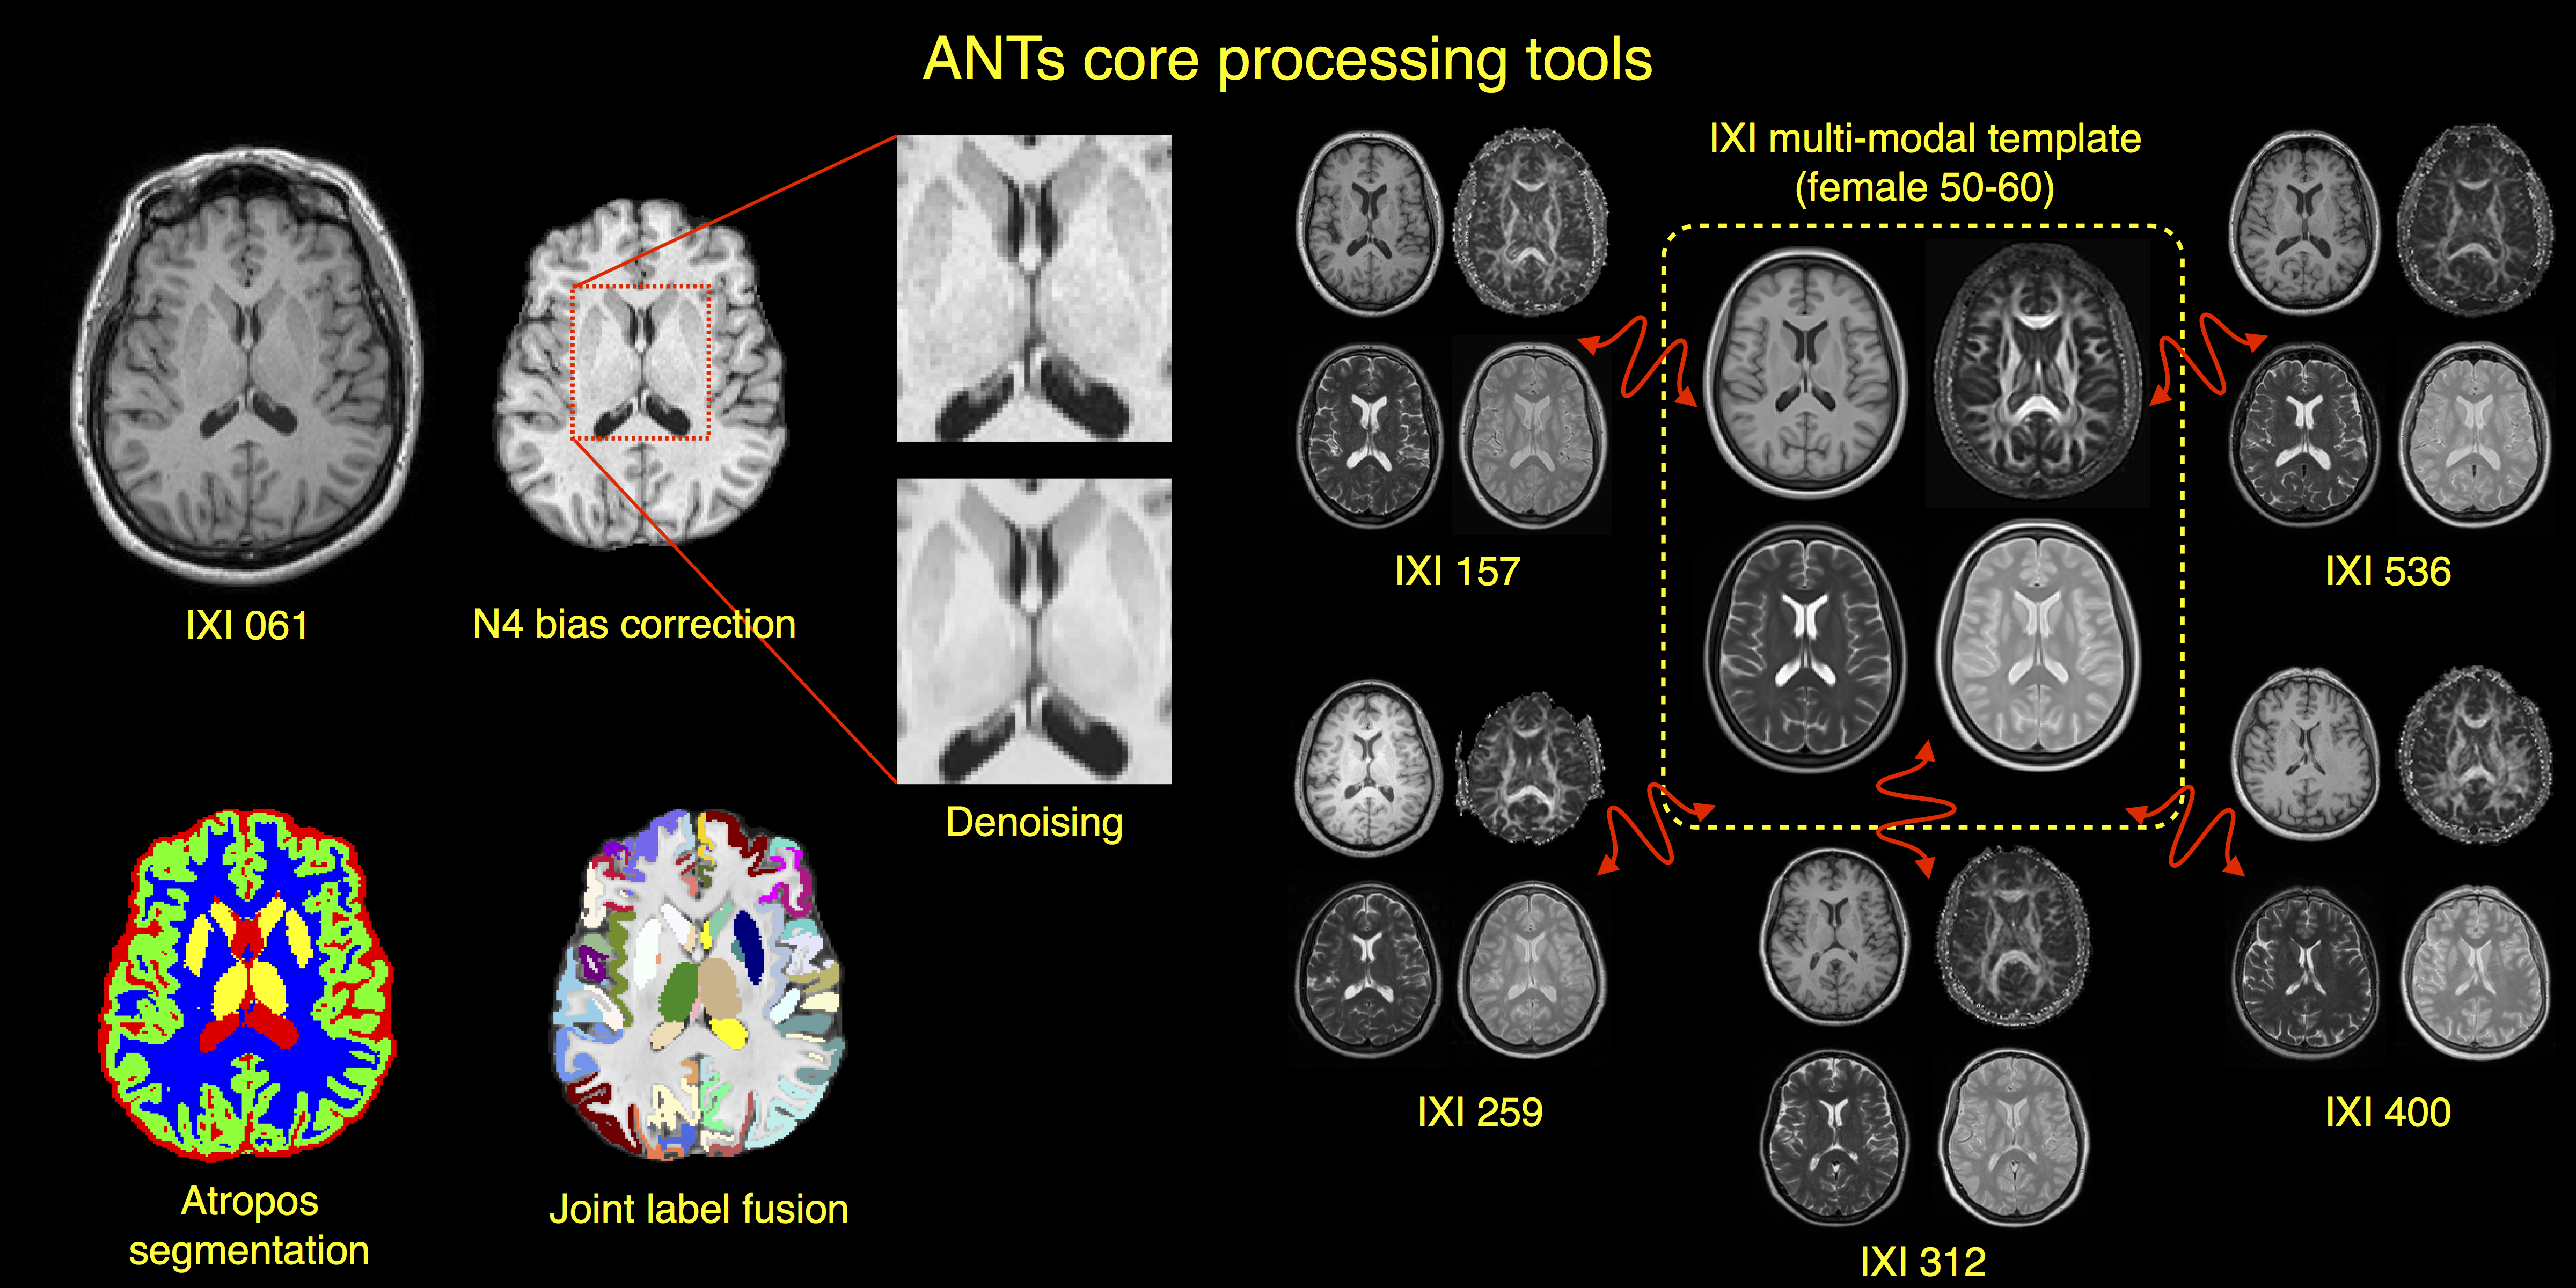
\includegraphics{Figs/coreANtsToolsNeuro.png}
\caption{Core processing tools that have made the ANTs package one of
the most popular neuroimaging toolkits. Fundamental processing tasks
such as image registration, template generation, bias correction,
denoising, intensity-based segmentation, and joint label fusion are
extremely well-performing software components which have been utilized
for neuroimaging tasks such as brain extraction and cortical thickness
estimation. The target applications of these core tools have an
immediate analog for lung-specific tasks such as lung and lobe
segmentation.}
\end{figure}

All of these tools have been wrapped in easy-to-use, well-documented
shell scripts. For example, the ANTs cortical thickness pipeline, as
outlined in {[}12{]}, comprises four major steps: (1) bias correction,
(2) brain extraction, (3) $n$-tissue segmentation, and (4) cortical
thickness estimation. Each step requires its own set of ANTs tools with
appropriately tuned parameters. To maximize the utility of the pipeline
for the interested user, in {[}12{]} we provide all the necessary
programs (properly tuned) with a minimal set of input data required to
obtain good results for common data. The result is an easy-to-use script
that can be invoked by the programmer and non-programmer alike to obtain
the desired processed data which outperforms the current
state-of-the-art {[}12{]}. An example command call for the ANTs cortical
thickness pipeline is:

\begin{Shaded}
\begin{Highlighting}[]
  \CommentTok{# ANTs processing call for a single subject}

  \NormalTok{$ }\KeywordTok{sh} \NormalTok{antsCorticalThickness.sh -d 3 \textbackslash{}}
                                \KeywordTok{-a} \NormalTok{IXI/T1/IXI002-Guys-0828-T1.nii.gz \textbackslash{}}
                                \KeywordTok{-e} \NormalTok{IXI/template/T_Template0.nii.gz \textbackslash{}}
                                \KeywordTok{-m} \NormalTok{IXI/template/T_template0ProbabilityMask.nii.gz \textbackslash{}}
                                \KeywordTok{-f} \NormalTok{IXI/template/T_template0ExtractionMask.nii.gz \textbackslash{}}
                                \KeywordTok{-p} \NormalTok{IXI/template/Priors/priors%d.nii.gz \textbackslash{}}
                                \KeywordTok{-o} \NormalTok{IXI/ANTsResults/IXI002-Guys-02828-}
\end{Highlighting}
\end{Shaded}

This approach to reducing the steep learning curve associated with many
processing pipelines has several benefits. Bash is an extremely common
command language that permits large-scale processing. Thus, running
several jobs on a cluster infrastructure is straightforward with this
approach. Such scripts are readable by the interested user who can glean
parameters as well as manually make changes.

\subsubsection{3(c.2) \textbf{Specific Aim 1:} To develop ITK-Lung, a
set of open-source software tools for CT, 1H, and 3He pulmonary
computational
analysis}\label{c.2-specific-aim-1-to-develop-itk-lung-a-set-of-open-source-software-tools-for-ct-1h-and-3he-pulmonary-computational-analysis}

The envisioned open-science tool set for pulmonary image analysis
consists of software, processed data to illustrate the use of the
software, and the ability to evaluate and visualize user-generated
results. With this comprehensive offering, the goal of this project is
to help the pulmonary imaging research community on a much deeper level
than simply providing a set of programs. In order to facilitate
engagement on the part of the community, we are proposing a multi-prong
offering with ITK-Lung. The main componenent will be the core tool set
described in Sub-Aim 1a which would permit large-scale processing of
multi-modal pulmonary image data. To illustrate the use of the software,
allow for processing of other public and private data sets, and provide
baseline data for algorithmic comparison, we plan to release CT and 1H
MRI annotated atlas libraries, corresponding templates, and
data-generating scripts as described below. The third component will be
significant extensions to the well-known ITK-SNAP software for an
enhanced user experience through a full featured graphical user
interface to support interactive parameter tuning and an extensive suite
of tools for evaluation and visualization of user-processed results.

\textbf{3(c.2.1) Sub-Aim 1a will expand the ITK/ANTs open-source
libraries by implementing currently unavailable lung-specific
algorithms.} Analogous to the neuroimaging tasks described earlier,
several algorithmic categories exist for lung image analysis which, as
we have noted previously, do not exist in any comprehensive, publicly
available package. This is in spite of the fact that new algorithms for
lung image analysis are frequently reported in the literature. An
extensive survey concentrating on the years 1999--2004 is given in
{[}59{]} which covers computer-aided diagnosis of lung disease and lung
cancer in CT (i.e., detection and tracking of pulmonary nodules) and
provides an overview of the many relevant segmentation methods for
pulmonary structures. Although many algorithms existed at the time,
continued technical development has only increased the number of
available algorithms. However, despite the continued \emph{reporting} of
pulmonary image analysis algorithms, there is no corresponding increase
in algorithmic \emph{availability}. \emph{Additionally, a key problem in
the pulmonary image analysis community is that the lack of publicly
available tools translates directly into a lack of baseline performance
standards with which researchers can compare their own algorithms
{[}60{]}. This project constitutes a specific and overdue response to
this major deficiency in the field.}

\begin{figure}[htbp]
\centering
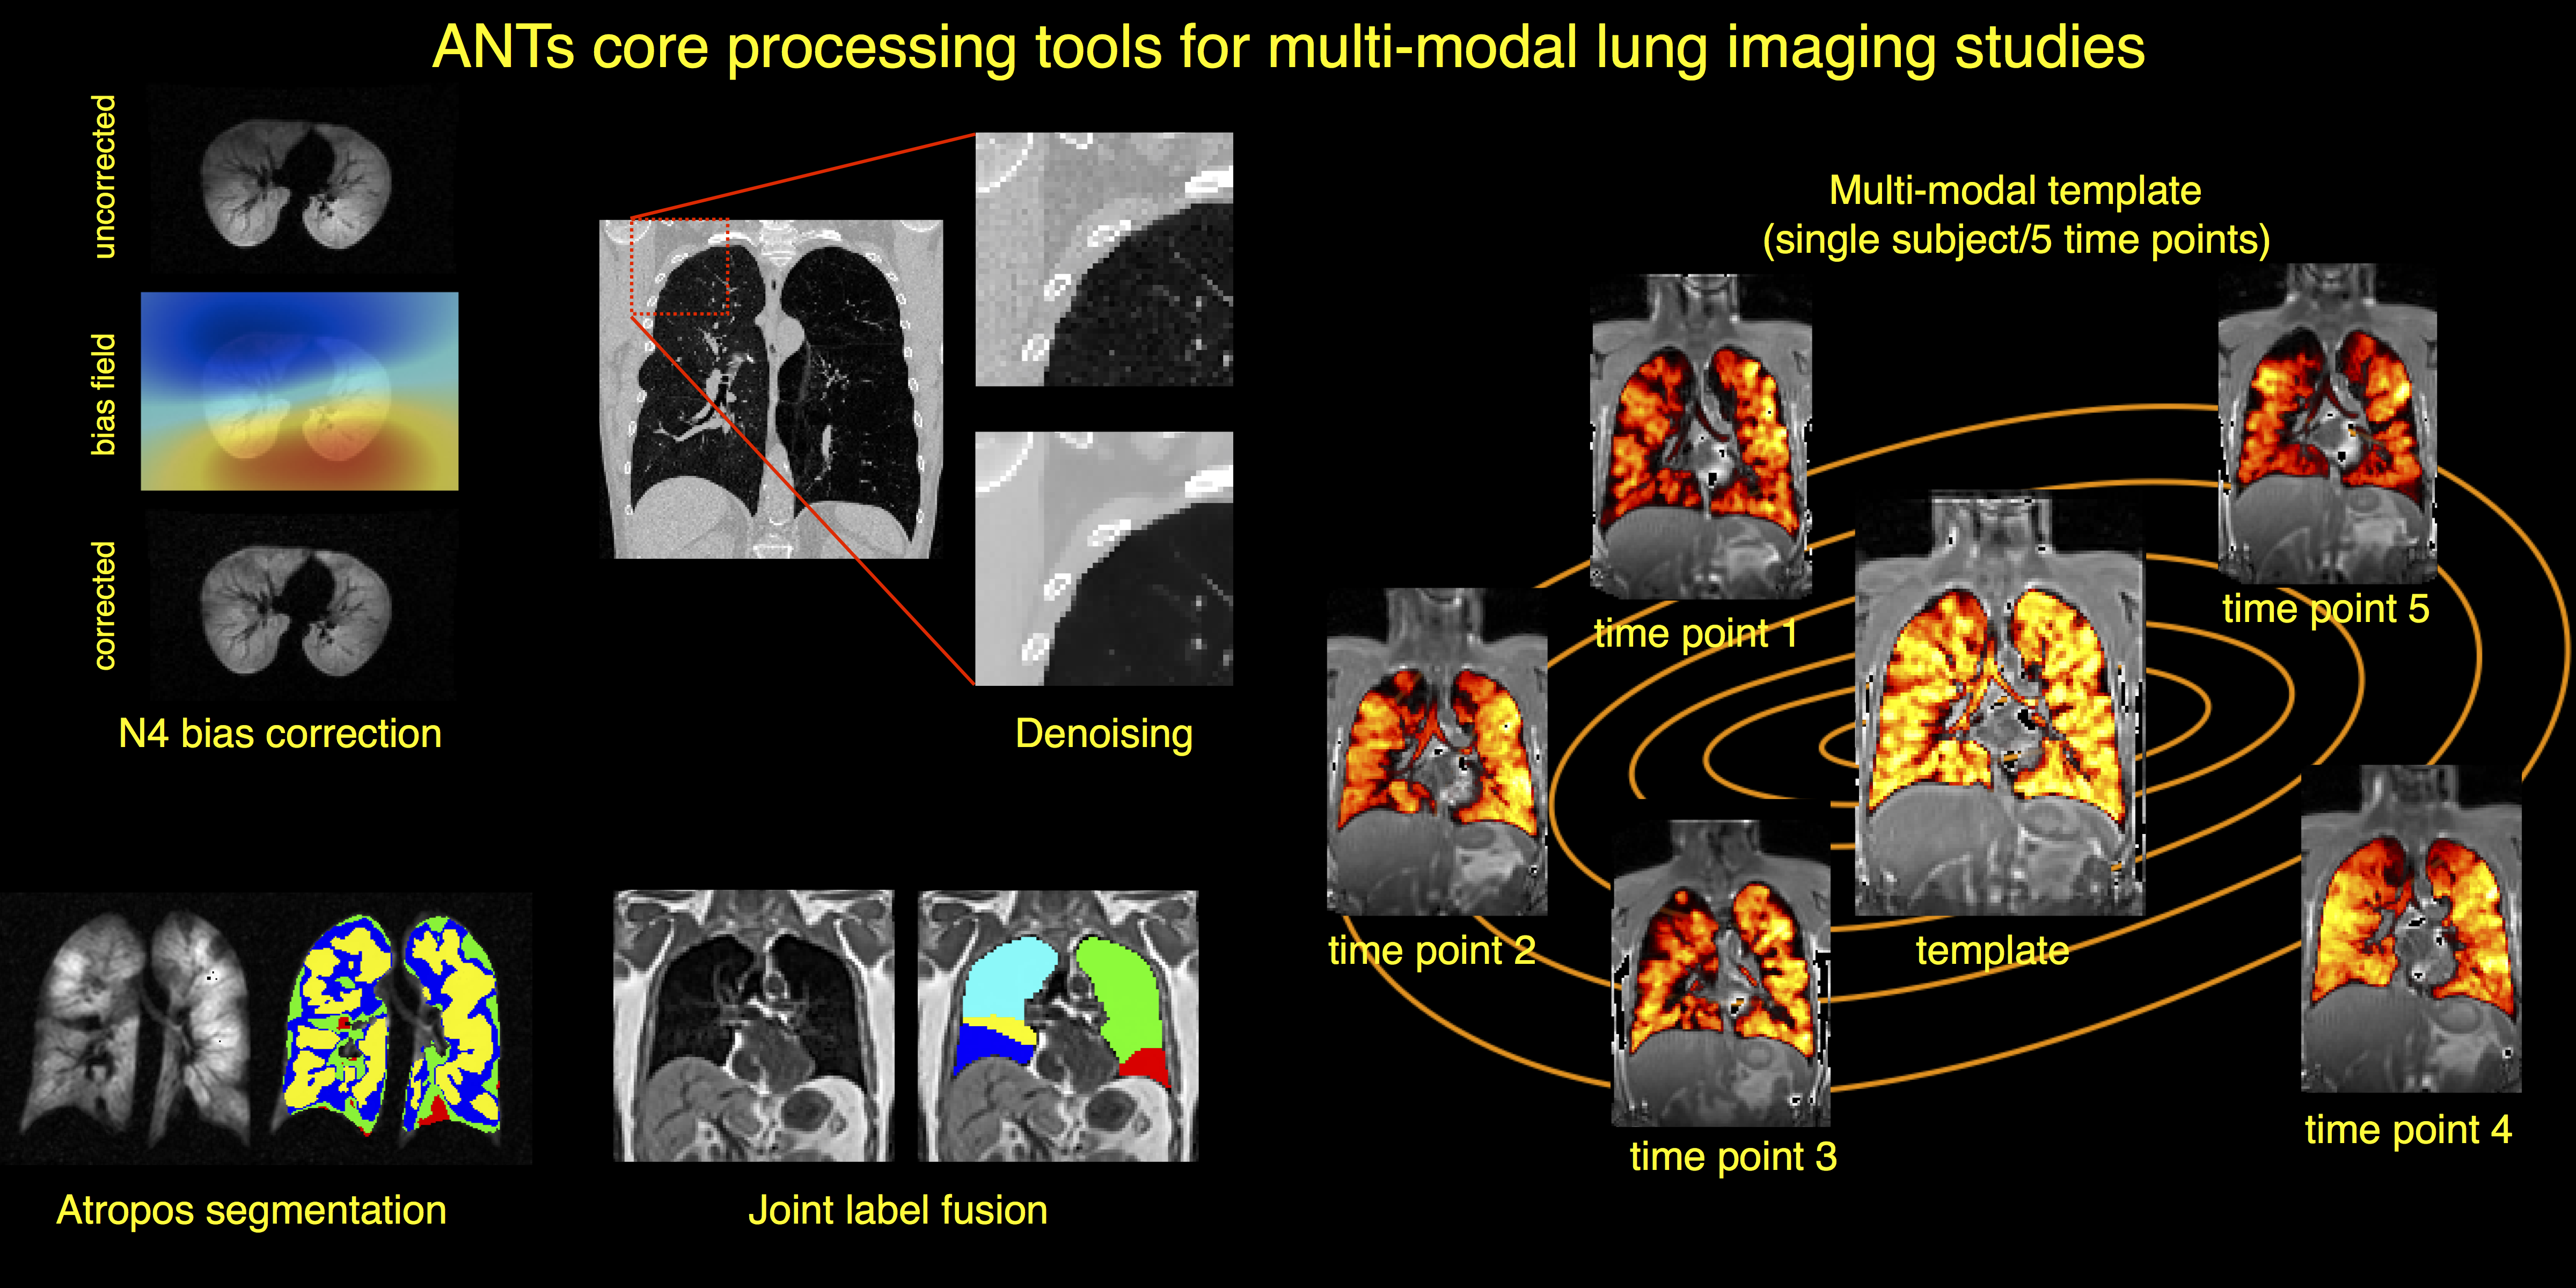
\includegraphics{Figs/coreANtsToolsLung.png}
\caption{Using ANTs core processing tools, our team has developed
several lung-specific extensions such as ventilation-based segmentation,
lung and lobe estimation, and multi-modal pulmonary template building.
Although each of these extensions requires significant additional
development and tuning, a robust and generic software foundation ensures
that these extensions are of high quality and are readily adapted to the
pulmonary image domain.}
\end{figure}

\emph{A primary impetus for this project is that, through extension and
continued development of ANTs and ITK functionality, we can make a
significant impact for the pulmonary imaging research community in both
basic science and clinical workflows by developing lung-specific
algorithms which are easy to use as we have done for the neuroimaging
community.} The following list comprises core functionality for CT
analysis that would be incorporated into ITK-Lung in addition to further
enhancements to registration and segmentation capabilities described in
preliminary work:

\begin{itemize}
\itemsep1pt\parskip0pt\parsep0pt
\item
  whole lung differentiation from the chest wall (e.g., {[}61--64{]}),
\item
  bronchial structure extraction (e.g., {[}65, 66{]} and the many
  submissions to the recent Extraction of Airways from CT (ExACT)
  challenge of the 2nd International Workshop on Pulmonary Image
  Analysis {[}67{]}),
\item
  vasculature segmentation (e.g., {[}68, 69{]}),
\item
  lobe and/or fissure detection (e.g., {[}70, 71{]}),
\item
  feature extraction and classification (e.g., {[}72--74{]}), and
\item
  nodule detection (e.g., {[}75{]} and the many submissions to the
  Automatic Nodule Detection (ANODE09) challenge of the 2009 CAD
  Conference of SPIE Medical Imaging {[}76{]}).
\end{itemize}

Although this list is restricted to CT image analysis, inclusion of
additional techniques specific to other modalities has additional
benefit and are planned for this project (cf Table 1). Using ANTs core
tools, we have produced several lung-specific algorithms for core tasks
such as:

\textbf{Atlas-based lung segmentation.} Identification of anatomical
structure in MRI is often a crucial preprocessing step for
quantification of morphological features or ventilation information from
functional images. Quantitative regional analysis often requires the
identification of lung and lobar anatomy. Although much algorithmic
research for lung segmentation has been reported in the CT literature
{[}77{]}, co-opting such technologies is complicated by MRI-specific
issues such as RF coil inhomogeneity, presence and resolution of
structural detail, and the absence of a physically-based intensity
scaling.

We recently proposed a multi-atlas approach for automatically segmenting
the left and right lungs in 1H MRI {[}47{]}. Multi-atlas approaches to
segmentation have proven highly successful in neuroimaging {[}43, 51{]}
and these methods translate readily to the pulmonary domain. Whereas
many current strategies for lung image segmentation employ low-level
processing techniques based on encodable heuristics, consensus-based
strategies, in contrast, optimize the prior knowledge applied to a
specific segmentation problem (cf Figure 3). The evaluation of our
proposed method {[}47{]} demonstrated excellent performance with Jaccard
overlap measures for the left and right lungs being $0.966 \pm 0.018$
and $0.970 \pm 0.016$, respectively. Further work for this project
includes extension to CT datasets with a particular emphasis on
segmentation in the presence of lung pathology which will incorporate
the data from the proposed multi-atlas CT library .


\begin{table}[!t]
  \small
   \centering
    \begin{tabular*}{0.75\textwidth}{c @{\extracolsep{\fill}} ccc}
    \toprule
    {\bf Functionality} & {\bf CT} & {\bf 1H MRI} & {\bf 3He MRI}\\
    \cmidrule[1pt](lr){1-4}
    spatial normalization & { \checkmark } & { \checkmark } & { \checkmark } \\
    template generation & { \checkmark } & { \checkmark } & { \checkmark } \\
    lung segmentation & { \checkmark } & { \checkmark } & {  } \\
    lobe segmentation & { \checkmark } & { \checkmark } & {  } \\
    airway segmentation & { \checkmark } & { } & {  } \\
    vessel segmentation & { \checkmark } & { } & {  } \\
    functional segmentation & { \checkmark } & {  } & { \checkmark } \\
    nodule detection & { \checkmark } & {  } & {  } \\
    feature indices & { \checkmark } & {  } & { \checkmark } \\
    \bottomrule
   \end{tabular*}
 \label{table:algorithms}
 \caption{Specific outline of basic functionality proposed for development and evaluation
 in the project
 categorized by modality.  One of the motivations for the collaborative use
 cases as a specific aim is the inevitability that other lung-specific
 algorithmic needs will be identified and will be added to the functionality
 developed and offered as part of this project.  It should also be noted that
 some modality-specific modifications will be required.  For example,
 our lobe estimation approach works well for 1H MRI where no internal anatomical
 features are available for refinement.  This lobe estimation strategy can be directly applied to CT in providing
 spatial prior maps for subsequent subject-specific refinement.
 }

\end{table}


\textbf{Atlas-based lobe estimation.} For regional investigation of
certain lung pathologies and conditions, it is often useful to quantify
measurements of interest within more localized regions, such as the
lobes. However there is little (if any) usable information in 1H MRI for
image-based lobar segmentation which has led to alternative geometric
subdivisions which are ad hoc, non-anatomical, and do not adequately
address intra- and inter-subject correspondences. However, we can take
advantage of inter-subject similarities in lobar geometry to provide a
prior-based estimation of lobar divisions using a consensus labeling
approach (cf Figure 3).

To generate the lobe segmentation in a target 1H or CT lung image, we
first generate a binary whole lung mask using the whole lung atlas-based
estimation. We then register a set of CT lung masks which have beeen
expertly annotated (as part of the multi-atlas library) to the target
binary lung mask using the B-spline SyN registration approach described
earlier {[}11{]}. Subsequently, we warp the set of CT lobe labels to the
target image using the CT mask-to-target mask transformation. This
process will be illustrated publicly as part of the project using the
open-data multi-atlas CT library created as part of Sub-Aim 1b.

Since we have no intensity information inside the target lung mask and
CT atlas lung masks, we use a simply majority voting strategy to
generate the optimal labeling for the target image. Following the
majority voting, we remove any labelings outside the lung mask and
assign any unlabeled voxels with the label closest in distance to that
voxel. This methodology is more thoroughly described in {[}47{]} where
we showed that lobar overlap measures in 1H MRI were on par with
state-of-the-art CT methods where fissure information is actually
visible (left upper: $0.882 \pm 0.059$, left lower: $0.868 \pm 0.06$,
right upper: $0.852 \pm 0.067$, right middle: $0.657 \pm 0.130$, right
lower: $0.873 \pm 0.063$). We will extend this framework to pulmonary CT
in providing spatial prior probability maps augmented by image-specific
CT data features as fissures, airways, and blood vessels for
data-driven, subject-specific lobe segmentation {[}71{]}.

\textbf{Ventilation quantification.} Automated or semi-automated
approaches for classifying areas of varying degrees of ventilation are
of potential benefit for pulmonary functional analysis. In {[}35{]}, we
presented an automated algorithmic pipeline for ventilation-based
partitioning of the lungs in hyperpolarized 3He and 129Xe MRI. Without
ground truth data for evaluation, we used a consensus labeling approach
{[}78{]} to simultaneously estimate the true segmentation from given
``raters'' which included the segmentation from our automated approach
and the manual tracings of three trained individuals. In terms of
combined specificity and sensitivity, our automated algorithm
demonstrated superior performance with the added benefit of being
reproducible and less time-consuming. Since the initial development, we
have continued to improve this segmentation pipeline by incorporating an
iterative bias-correction/segmentation estimation scheme. An additional
component that improves results is an ANTs-based implementation of the
patch-based denoising protocol described in {[}48{]}.

\textbf{Multi-modal lung template construction.} Although the template
construction algorithm described in {[}19{]} is, as pointed out earlier,
frequently applied to T1-weighted brain data, it is sufficiently general
such that it can potentially be applied to pulmonary data. Also, new
innovations in diffeomorphic registration technology has led to a
Symmetric Normalization B-spline variant which will be extended and
refined to provide accurate normalizations {[}11{]} for pulmonary data
{[}18{]}.

\textbf{Feature indices.} Imaging biomarkers for characterizing
emphysema in CT have have been well researched, although there are ample
opportunities to refine these methods as well as to introduce more
advanced approaches. Examples of the latter include texture analysis for
identifying the centrilobular and groundglass opacities and fractal and
connectivity approaches to differentiate centrilobular from panlobular
emphysema. The available indices for CT image analysis can roughly be
divided into those that characterize the pulmonary parenchyma:
volumetric tissue (e.g., {[}79, 80{]}), distribution of low attenuation
areas (LAA) (e.g., {[}81, 82{]}), cooccurrence and run-length matrix
features (e.g., {[}72, 83{]}), attenuation statistics (e.g., {[}84,
85{]}), deformation measures (e.g., {[}86, 87{]}), and stochastic
fractal dimension features (e.g., {[}72, 85{]}); and those that
characterize the airways (e.g., {[}88--90{]}). The former are important
for subjects with an emphysematous component of disease, whereas the
latter are important for subjects with a bronchitic component of
disease. \emph{An important component of this project is that many of
these measurements can also be directly applied to discriminative
analysis using 3He MRI for a variety of lung diseases.} These indices
can also be studied not only at any particular single time point, but
also for changes with time. The addition of quantitative morphologic
measurements of the airways provides an assessment of the contribution
of airway changes to chronic lung disease.


\begin{table}[!t]
  \small
  \begin{minipage}{0.33 \linewidth}
   \vspace{2mm}
   \centering
    \begin{tabular}[t]{c}
    {\bf Volumetric Tissue Indices}  \\
    \cmidrule[1pt](lr){1-1}
    lung volume   \\
    lobar volume  \\
    surface area  \\
    surface area to volume ratio  \\
    total lung weight  \\
    tissue/airspace volumes of lung \\
    inspiration vs. expiration$^*$ \\
    \\
    {\bf Airway Indices} \\
    \cmidrule[1pt](lr){1-1}
    airway luminal diameter and area  \\
    airway wall thickness  \\
    percentage wall area   \\
    thickness to diameter ratio  \\
    airway branch angles  \\
    airway segment length  \\
    airway wall volumes (segmental and total)$^*$ \\
    inspiration vs. expiration  \\
    \\
    {\bf Distribution of LAA Heterogeneity}  \\
    \cmidrule[1pt](lr){1-1}
    10 partitions (std of $15^{th} \%$)  \\
    slopes of density mask curves  \\
    $\%$ size distribution of LAA areas \\
    volumetric cluster analysis \\
    inner core vs. outer rind \\
    inspiration vs. expiration$^*$ \\
    \\
   \end{tabular}
   \end{minipage}
  \hspace{0cm}
  \begin{minipage}{0.33 \linewidth}
   \vspace{-8mm}
    \centering
    \begin{tabular}[t]{c}
    {\bf Cooccurrence Matrix Texture Indices}  \\
    \cmidrule[1pt](lr){1-1}
    energy  \\
    inertia  \\
    contrast  \\
    entropy  \\
    correlation  \\
    inverse difference moment \\
    cluster shade$^*$ \\
    cluster prominence$^*$ \\
    Haralick's correlation$^*$ \\
    \\
    {\bf Run-length Matrix Texture Indices}  {} \\
    \cmidrule[1pt](lr){1-1}
    short run emphasis  \\
    long run emphasis   \\
    grey level non-uniformity   \\
    run-length non-uniformity  \\
    run percentage  \\
    low grey level run emphasis$^*$ \\
    high grey level run emphasis$^*$ \\
    short run low grey level emphasis$^*$ \\
    short high grey level run emphasis$^*$ \\
    long run low grey level emphasis$^*$ \\
    long high grey level run emphasis$^*$ \\
    inspiration vs. expiration$^*$\\
    \\
    \end{tabular}
   \end{minipage}
  \hspace{0cm}
  \begin{minipage}{0.33 \linewidth}
   \vspace{0mm}
    \centering
    \begin{tabular}[t]{c}
    {\bf Attenuation Histogram Statistics}  \\
    \cmidrule[1pt](lr){1-1}
    attenuation mean  \\
    attenuation variance  \\
    attenuation skewness  \\
    attenuation kurtosis  \\
    attenuation grey level entropy  \\
    regional variants  \\
    inspiration vs. expiration \\
    \\
    {\bf Deformation Indices}  {} \\
    \cmidrule[1pt](lr){1-1}
    Jacobian of lung displacement  \\
    lung deformation strain  \\
    \\
    {\bf Stochastic Fractal Image Statistics}\\
    \cmidrule[1pt](lr){1-1}
    mean  \\
    variance  \\
    skewness  \\
    kurtosis  \\
    grey level entropy  \\
    inspiration vs. expiration$^*$  \\
    \\
    {\bf Attenuation Mask Indices} \\
    \cmidrule[1pt](lr){1-1}
    HU density mask   \\
    $\%$ HU density mask  \\
    inspiration vs. expiration$^*$ \\
    \\
    \end{tabular}
   \end{minipage}
 \label{table:indices}
 \caption{Quantitative CT indices proposed for inclusion in the lung image analysis pipeline.  Whole lung, regional, and voxelwise measurements are included, as well as population-based comparisons and longitudinal analysis of all indices.  Indices marked with a `*' denote novel measures which have not been previously utilized in chronic lung disease assessment but have shown classification capability in other application domains.}
\end{table}


Table 2 provides an overview of these types of discriminative
measurements, many of which can be used for CT and 3He lung assessment.
We have already implemented many of these image features and have
contributed the result of our work to the Insight Toolkit (e.g., {[}91,
92{]}).

\textbf{Airway and vessel segmentation.} In describing the quantitative
CT lung indices, it was pointed out that lung airway morphology has been
previously utilized as a biomarker for disease characterization.
Additionally, there are other potential uses motivating the inclusion of
airway segmentation in any pulmonary image analysis toolkit. In an
evaluation of 15 airway segmentation algorithms {[}93{]} for the
Extraction of Airways from CT challenge held in 2009, the top 2
performers were the algorithms of {[}94{]} and {[}95{]} with the latter
being one of the more conservative algorithms and the former being more
prone to false positives. Our plan is to provide an implementation of
{[}94{]} and then augment this functionality with some of our previous
work {[}96{]} for removing leakage path candidates.

ITK has extensive functionality for segmentation of vessel-like
structures. Much of that work has been incorporated into comprehensive
packages such as the analysis and visualization Vessel Modeling ToolKit
(\url{http://www.vmtk.org}). For this project we will focus development
and refinement of these ITK capabilities for CT lung application in
segmenting the pulmonary vasculature.

\textbf{Nodule detection.} CT is used for screening of lung cancers
(i.e., pulmonary nodules) which currently requires human intervention
for the laborious and tedius task of manual scanning. Automated
detection methods could potentially save significant time and effort
which has inspired much research literature on the topic including
several commercial systems and specialized visualization hardware for
facilitating detection. In 2009, a nodule detection competition was held
for comparing performance of individual algorithms as well as their
combinations {[}76{]}. This competition included entries from both
academic institutions as well as a system from Philips (although, to our
knowledge, none are available for public use). The best performing
algorithm of that competition was based on the work presented in
{[}97{]} where a k-nearest neighbor classification employing local image
features is built from a large training data set. We plan to implement
this method potentially with some modifications based on our experience
with a more recent challenge dealing with segmentation of pathology
{[}20{]}.

\textbf{3(c.2.2) Sub-Aim 1b will provide two annotated multi-atlas
libraries, one for CT and another for 1H MRI.} The corresponding group
templates will also be provided along with the scripts to produce the
results using ITK-Lung. As a complement to the open-source software
provided in Sub-Aim 1a, we will generate atlas libraries for both CT and
1H MRI acquisitions. As indicated above, such atlases provide extremely
useful prior information for performing robust and accurate lung and
lobe segmentations within their respective modalities. Additionally, the
accompanying annotations provide an open-data platform for
quantitatively assessing other lung and lobe segmentation algorithms.
Both libraries will consist of $n=30$ different subjects to represent a
range of lung size and shape and will be annotated according to
modality. The CT atlas library will include lung, lobe, airway, and
vessel segmentations. The 1H MRI atlas library will include left/right
lung segmentations and lobar estimations {[}47{]}. Along with the
annotated data we will provide the scripts and documentation to allow
reproduction of the ITK-Lung results. Additionally, two group templates
{[}19{]} for the two atlas libraries, respectively, will be included as
part of these open data sets.

\textbf{3(c.2.3) Sub-Aim 1c will develop a graphical user interface
(GUI) for running ITK-Lung on user data and evaluating processed
results.} ANTs will be the workhorse toolkit for the registration
development effort in Aim 1, and the creation of a user-friendly GUI
enabling interactive access for the first time to ANTs functionality
will be a critical innovation toward a comprehensive registration
solution for imaging studies of the lung. The existence of the GUI will
not only open ANTs to users without programming experience---which is
expected to greatly expand its already considerable user base and in
turn further increase its impact on the field---but will also
significantly enhance the power of ANTs by allowing human/expert input
to interactively tune parameters and intelligently initialize as well as
steer the registration toward the solution that best satisfies both user
and algorithmic constraints. Equally important, the GUI will permit
qualitative and quantitative assessment of the results produced by
ITK-Lung as well as potentially other software, another much needed
capability not currently available to the general community. Based on
these considerations, we propose to base the GUI front-end to ITK-Lung
on the ITK-SNAP multi-platform, open-source tool for interactive
user-guided medical image segmentation and data visualization {[}98{]},
whose development is led by project investigator Paul Yushkevich.
ITK-SNAP provides an effective combination of semi-automatic
segmentation functionality based on active contours {[}99{]} and manual
delineation functionality, put together into a compact and easy-to-learn
GUI, that perfectly complements the automated segmentation functionality
proposed for development in this project. ITK-SNAP design emphasizes
interaction and ease of use, with the bulk of the development effort
dedicated to the user interface. ITK- SNAP has thousands of users (there
have been over 2000 downloads per month in the last year), and our 2006
paper on ITK-SNAP {[}98{]} has been cited over 1400 times (Google
Scholar) in the context of various biomedical domains. ITK-SNAP will
also be used in this project for manual labeling of the proposed lung
atlases; it is already used for this purpose by many investigators. Most
crucially, we believe that our track record with ITK-SNAP as well as
ANTs demonstrates our team's commitment to producing high-quality
research software and making it accessible to the wider research
community through open-source practices, intuitive user interfaces, and
outreach efforts. These strengths of the team will be applied to the
software and data developed in the course of this project.

Several features will be added to ITK-SNAP to enhance visualization and
quantitation for the registration and segmentation results of the
lung-specific algorithms developed in the project. Users will be able to
edit and annotate these segmentations, modify registration transforms,
and extract quantities both globally and regionally. Transforms will be
modifiable via manual annotations (clicking corresponding landmarks,
tracing curves, and/or painting regions) or by directly modifying
transform parameters. Quantitative parameters, such as volumes and
strain tensors, will be available through the ITK-SNAP interface.
Finally, existing ITK-SNAP functionality for segmentation visualization
will be extended to support evaluation of registration quality,
including a dashboard of performance metrics, linked cursors identifying
corresponding positions in multi-window configurations, and fused data
displays with adjustable blending. These proposed enhancements to the
software will be extremely useful to the general imaging research
community and not just those investigators targeted in this project.
Thus, the impact of this work will be both immediate and broad for
pulmonary-driven science and research.

\textbf{3(c.2.4) Software engineering.} Both ANTs and ITK-SNAP
development, based on a solid foundation provided by the Insight
Toolkit, utilizes open-source software engineering best practices, such
as the use of Git version management software for collaborative
development and easy branching and merging; use of a centralized
repository (SourceForge) for code, executable and data sharing; and use
of the CMake/CTest/CDash suite for cross-platform development, testing
and automatic builds. Virtual machines with different versions of
Windows, MacOS and Linux operating systems generate nightly builds and
execute test code, uploading a binary to the central SourceForge
repository. ANTs and ITK-SNAP are documented through video and text
tutorials, housed online on dedicated websites {[}13, 101{]}. A similar
infrastructure will be developed for the software resources proposed in
Aim 1.

\subsubsection{3(c.3) \textbf{Specific Aim 2.} Validate and disseminate
the developed ITK-Lung resources by leveraging use cases from a broad
network of partner investigators representing the state-of-the-science
in lung imaging
research}\label{c.3-specific-aim-2.-validate-and-disseminate-the-developed-itk-lung-resources-by-leveraging-use-cases-from-a-broad-network-of-partner-investigators-representing-the-state-of-the-science-in-lung-imaging-research}

This aim builds on the project team's long and successful track record
of collaboration with the general user community. In particular, the
investigator-driven studies presented below are carefully selected both
for their capacity to fully exercise the developed tools and to provide
a comprehensive representation of the various processing and analysis
tasks of interest to the community.

\textbf{3(c.3.1) Novel imaging biomarkers for Chronic Obstructive
Pulmonary Disease (COPD).} Co-investigator \textbf{Mike Shim} and his
group have been actively developing 3D hyperpolarized xenon-129
dissolved-phase MRI (HXe MRI) as a sensitive biomarker for accurately
characterizing phenotypes and severity of COPD. This protocol permits
regional mapping of ventilation and gas uptake by tissue and blood in
human lungs with single breath hold {[}102--104{]}. This project plans
to establish connectivity between these advanced HXe MRI imaging
signatures and important clinical outcomes of COPD to establish HXe MRI
as a novel clinical diagnostic tool. They anticipate that this new
biomarker tool will naturally lead to deeper mechanistic understanding
of COPD at the molecular-physiologic and clinical levels and support
identification of potential pathophysiologic derangement associated with
COPD and a new method to accurately predict therapeutic response to
current standard COPD therapies. Refinement of HXe MRI as a pulmonary
diagnostic tool is anticipated to encourage development of new clinical
interventions. HXe MRI is the first non-invasive imaging technique that
can provide regional information about three unique characteristics of
lung function: lung ventilation, size and connectedness of distal
alveolar airspaces, and HXe gas transfer from airspaces to red blood
cells. HXe MRI, therefore, is anticipated to overcome the limitation of
pulmonary function testing (PFT) which only provides physiologic
parameters of the lung as a whole unit, and High Resolution CT (HRCT)
which only provides anatomic characterization without physiologic
information. HXe MRI is anticipated to detect pathologic changes present
in COPD patients with high sensitivity and specificity previously
unattainable by current clinical standard (PFT and HRCT). Moreover, HXe
MRI can determine whether gas transfer abnormalities are due to impaired
ventilation or reduced gas-exchange, and thus provide new insights into
pathogenesis of COPD in individual patients.

Crucial to the success of establishing the utility of HXe MRI as a
sensitive biomarker for accurately characterizing COPD phenotypes is
quantification of imaging signatures in an automated and robust fashion.
Identification of ventilation dead space ($V_D$) for correlation with
GOLD classification will utilize the ventilation-based segmentation
functionality in ITK-Lung {[}35{]}. In order to determine lobar values
of HXe MRI, we will utilize the recently proposed lobar estimation
algorithm {[}47{]} that will be available for both proton MRI and CT

\textbf{3(c.3.2) Hyperpolarized gas imaging in children with asthma.}
Advances in rapid image sequencing methods have facilitated the
acquisition of high-quality hyperpolarized gas MR images in pre-school
children {[}105{]}. Furthermore improvements in image processing and
signal intensity analysis have made possible accurate measurements of
lung volume compartments {[}35{]}. Co-investigators \textbf{Gerry
Teague} and \textbf{Talissa Altes} are applying these innovations in
children with asthma to study whether the lung defect volume \% as
measured by hyperpolarized lung MRI correlates with a range of clinical
features. They hypothesize the ventilation defect volume \% would be
higher in children with severe asthma, and correlate not only with the
degree of airflow limitation, but indicators of asthma control,
treatment, and inflammation.

Precise measurement of ventilation volumes by hyperpolarized noble gas
MRI not only has the potential to resolve the spatial and temporal
characteristics of gas distribution in children with asthma, but could
also expand clinically relevant information in regards to asthma
severity and its features. In the past simple computer-assisted systems
{[}106{]} or hand counts of visual defects were used to estimate the
ventilation defect volume {[}107{]}. Development of more advanced
techniques (in terms of acquisition and analysis) will facilitate rapid
conversion of complex hyperpolarized gas signal data into volume
compartments for clinical applications.

Absolutely crucial to the advanced techniques being developed by
Dr.~Teague and his group are sophisticated image analysis tools like the
ones being proposed. For example, our ventilation-based segmentation
method is already being used to determine volumetric compartments based
on lung function. Additional ``cleaning'' necessary for these data
include denoising techniques {[}48{]} implemented and made available in
ANTs. Lobe estimation will be possible by refining the techniques
originally described in {[}47{]}.

\textbf{3(c.3.3) Characterization of COPDGene cohort by hyperpolarized
gas (HP) MRI.} Co-investigator \textbf{Rahim Rizi} is leading a study of
lung function and structure in COPD using HP MRI. Once inhaled, this gas
can tell the researcher how well specific lung regions replace the air
during the normal breathing cycle (Fractional Ventilation, FV), how much
oxygen is in the airspaces (Oxygen Tension, PAO2), and if the normal
spongy tissue structure has been compromised in lung disease (Apparent
Diffusion Coefficient). Subjects will include those at risk for lung
disease, and those displaying mild and moderate COPD. Subjects will be
mostly drawn from the well-characterized population currently enrolled
in the COPDGene trial (10,000 subjects overall) such that standard
clinical images (End Inspiration and End Expiration CT) and Pulmonary
Function Tests (PFTs), as well as genetic sequencing, will already have
been done. Each subject will be imaged twice during the course of the
five-year study, and regional features will be compared between the CT
and MRI images to the genetic markers, changes in clinical measurements,
and patient quality of life.

The proposed study will generate non-invasive biomarkers of COPD
progression derived from minute, short-term alterations in lung function
and microstructure. Due to the excellent safety profile of MRI, these
metrics will be appropriate for use in novel, flexible study designs.
Perhaps most importantly, this research will enhance understanding of
the natural history of COPD. In doing so, it will provide a vital
supplement to ongoing efforts to identify COPD subtypes by adding
substantial physiologic detail to descriptions of this disease. The
overall goals of the study experiments are: a) to develop imaging
markers that better identify early COPD; b) to develop tests that
predict health deterioration due to COPD; c) to determine if specific
patterns of disease progression are associated with genetic markers
identified in the larger COPDGene study; and d) to determine if disease
progression is in part caused by excessive stretch in regions of the
lung next to blocked-off areas unable to inflate normally.

More than 200 million people suffer from COPD worldwide. Yet effectively
assessing the progression of this increasingly prevalent disease and
monitoring its response to treatment remain problematic. Hyperpolarized
gas MRI can help rectify these issues by providing sensitive
measurements of lung physiology and microstructure, but its adoption by
clinicians and investigators has been slow. In contrast, CT-based
methods for measuring emphysema, airway wall thickening, and expiratory
air trapping have become common in COPD clinical studies. There are
several reasons for this: CT is more accessible, its images possess
excellent spatial resolution, and quantification of these images is
currently superior. However, most CT-based parameters have only an
indirect relation to physiology, and the modality exposes patients to
ionizing radiation. Both of these shortcomings can be addressed by HP
gas MRI. Consequently, the study seeks to more fully exploit the
clinical potential of HP gas MRI by optimizing and testing parameters
for the regional assessment of COPD patients and symptomatic smokers.

A novel multi-breath HP MRI technique allows for the simultaneous
measurement of fractional ventilation (FV), regional partial pressure of
oxygen (PAO2), and apparent diffusion coefficient (ADC). Obtaining all
three parameters in a single scan reduces the necessary amount of
imaging gas while increasing accuracy by correcting artifacts associated
with collateral ventilation and the slow filling of parenchyma in
diseased lungs. Each of these metrics allows for the investigation of a
vital aspect of lung disease progression and their comparison with the
current CT-based standard of care will help to more clearly understand
different features and phenotypes of COPD.

The proposed image analysis software will be central to the successful
conduct of the following tasks necessary to establish the goals of this
study:

\begin{itemize}
\itemsep1pt\parskip0pt\parsep0pt
\item
  Registration of the multibreath/multislice gas MRI images of the whole
  lung consisting of a minimum of seven time points
\item
  Registration and analysis of inspiratory and expiratory CT for airway
  changes to assess airway collapsibility and remodeling and other CT
  markers
\item
  Registration and analysis of inspiratory and expiratory CT with MRI to
  study the similarities and differences of the two modalities in
  phenotyping the COPD population
\item
  Registration of the follow-up MRI and CT images (two years) to
  determine if disease progression is in part caused by excessive
  stretch in regions of the lung next to blocked-off areas unable to
  inflate normally (based on the baseline MRI and CT)
\end{itemize}

\textbf{3(c.3.4) Advanced image analysis of CT for early diagnosis and
prognosis of bronchiolitis obliterans syndrome (BOS) in lung transplant
patients.} Co-investigators \textbf{Eduardo Barbosa} and \textbf{Warren
Gefter} are conducting a retrospective study of more than 300 lung
transplant patients to advance the early diagnosis of BOS. Lung
transplantation is an established treatment for end-stage, irreversible
pulmonary disease, particularly due to COPD and interstitial lung
disease (ILD). While continued improvements in surgical techniques and
immunosuppressive medications have reduced the complication rates and
increased short-term survival after the procedure, chronic allograft
rejection due to bronchiolitis obliterans (a fibrous obliterative
disease of bronchioles representing the histological hallmark of chronic
rejection and resulting in obstructive pulmonary physiology) remains the
major cause of morbidity and mortality after six months following
transplantation. Bronchiolitis obliterans currently represents the
greatest limitation to long-term survival after lung transplantation.
While the diagnosis of bronchiolitis obliterans is a pathologic one and
therefore requires invasive biopsy, the distribution of disease is
patchy, with focal areas of abnormality surrounded by normal lung, and
consequently even biopsies may fail to demonstrate the diagnosis. For
these reasons, the International Society for Heart and Lung
Transplantation has recommended using declining spirometry, termed
bronchiolitis obliterans syndrome (BOS), as a surrogate marker of
chronic allograft rejection. In clinical practice, the diagnosis of BOS
is suspected based on an unexplained decline in lung function (measured
by PFT, of greater than 20\% of baseline FEV1) and worsening cough and
dyspnea, in the absence of other explanations such as pulmonary
infection or congestive heart failure. MDCT plays an important role by
demonstrating low attenuation areas representing air trapping,
particularly on expiratory images, which correlate with the presence of
bronchiolitis obliterans. Prior studies reported limited sensitivity for
the early diagnosis of bronchiolitis obliterans; however these utilized
semi-quantitative or qualitative assessment of air trapping in
non-volumetric data sets. This study aims to assess whether more
advanced, fully automated imaging analysis can detect early BOS prior to
development of clinically apparent disease.

PFT is the current reference standard for diagnosis of BOS; however, by
the time PFT abnormalities beyond the threshold of BOS diagnosis ensue,
the disease is already manifest and is not reversible with existing
therapies. It is conceivable that sophisticated analysis of CT,
including quantitative attenuation masks in inspiratory and expiratory
datasets, image registration and texture based feature extraction may
allow earlier detection of BOS in the preclinical phase, potentially
generating surrogate biomarkers for drug trials and earlier
prognostication.

Application of the proposed advanced software tools and algorithms in
this project for quantitative analysis of CT images in lung
transplantation patients will be crucial to enable computation of an
array of first and second order statistics which would capture not only
attenuation maps but also regional deformation and texture based
features. In combination, this would allow multiparametric statistical
modeling that may predict which patients will develop BOS before PFT
abnormalities beyond the diagnostic threshold ensue. Such tools will be
extended to other diffuse lung diseases, potentially generating new
biomarkers for diagnosis, prognostication and therapeutic trials.

\textbf{3(c.3.5) Comparison of automated multi-modality registration
methodologies to manual registration for assessing lung CT bronchial
morphologic changes and hyperpolarized helium MR ventilation defects in
asthma patients: Can automation speed the work flow for combining
structure and function using airways measures from CT and ventilation
measures from HP gas MRI?} Our collaborators \textbf{Sean Fain} and
\textbf{Mark Schiebler}, \textbf{University of Wisconsin}, are part of
the SARP (Severe Asthma Research Program) team developing imaging
biomarkers of asthma severity for predicting asthma exacerbation. The
approach of finding airway abnormalities that correlate with ventilation
defects is viable only with the availability of robust image
registration across the two modalities. Furthermore, translation to the
clinic will require standardized implementations across sites, and the
project's open-source platform is ideal for this purpose.

\textbf{3(c.3.6) Validation of voxel-based ventilation CT.} Our
collaborator \textbf{Jim Wild}, \textbf{University of Sheffield}, has
been active in the field of methods development for quantitative
pulmonary imaging and its clinical translation for more than a decade.
Relevant to this project, his group requires advanced registration
capabilities to validate a novel CT technique for obtaining
high-resolution images of pulmonary ventilation. In addition, there is
need within his research for multi-modality registration of pulmonary CT
and MRI images as well as segmentation of key lung structures as part of
standard processing workflows.

\textbf{3(c.3.7) Deep functional phenotyping of COPD.} Our collaborator
\textbf{Hans-Ulrich Kauczor}, \textbf{University Medical Center
Heidelberg}, is leading the COSYCONET (German COPD and Systemic
Consequences--Comorbidities Network) study, the world's first
prospective multicenter trial comparing proton MRI and CT imaging for
characterizing COPD, with the latter modality serving as the reference
standard. Automated image registration and segmentation will play a
vital role in defining the quantitative CT (air trapping, airway
collapsibility and remodeling, and pulmonary blood volume and vascular
pruning) and MR (air trapping, perfusion volume defects, and hypoxic
vasoconstriction) imaging biomarkers that form the basis for the study.

\textbf{3(c.3.8) Longitudinal imaging follow-up in COPD and lung cancer
Our collaborator }Joon-Beom Seo\_\_, \textbf{Asan Medical Center},
directs the imaging component of the Korean Obstructive Lung Disease
(KOLD) cohort study, which has collected over 1000 COPD cases from 17
participating centers with repeated imaging since 2005. He also leads a
national lung cancer radiomics project that has accrued 800 cases to
date. In both studies, robust image registration is essential to
tracking changes over time, and segmentation is an additional
requirement to support automated lesion delineation for the cancer
project.

\textbf{3(c.3.9) Advanced image processing pipelines for MR image-guided
pulmonary therapy decisions and support.} Our collaborator \textbf{Grace
Parraga}, \textbf{University of Western Ontario}, has been at the
forefront of MR imaging of lung structure and function since 2005. A
major challenge hampering widespread translation of current pulmonary
imaging advances is the lack of precision in their interpretation,
thereby complicating the planning and guiding of targeted therapies. The
project's software tools will enable the development of robust analysis
pipelines for the translation of in vivo imaging biomarkers in an open
and consistent manner across platforms and centers. This work, carried
out in collaboration with industrial partners, will support patient
phenotyping and stratification to therapy as well as measurement of
longitudinal changes and response to therapy.

\textbf{3(c.3.10) Functional MR imaging of the lungs using
hyperpolarized and inert gases.} Our collaborator, \textbf{Mitchell
Albert}, \textbf{Thunder Bay Regional Research Institute}, has been
advancing the use of inert fluorinated gases that can be breathed
continuously in order to measure indicators of wash-in, wash-out and air
trapping with dynamic imaging protocols. To compute the wash-in and
wash-out time constants on a pixelwise basis, access to accurate and
reliable image registration tools will be essential.

\textbf{3(c.3.11) Multimodality imaging studies of pulmonary diseases.}
Our collaborator, \textbf{Edwin van Beek}, \textbf{University of
Edinburgh}, has been conducting various multimodality studies, including
the evaluation of pulmonary fibrosis using both gadolinium-enhanced MRI
and contrast-enhanced CT perfusion imaging, and the assessment of lung
nodules using PET-CT and CT perfusion imaging. These relatively new
techniques would benefit from quantitative analysis of contrast
enhancement, and advanced image registration and segmentation
capabilities will both be necessary toward this end.

\textbf{3(c.3.12) Computational imaging biomarkers for diverse thoracic
malignancies.} Our collaborator, \textbf{Yoshiharu Ohno}, \textbf{Kobe
University}, leads a comprehensive program of multi-modality imaging
(CT, MRI, PET, molecular imaging) research on lung cancer, COPD, ILD,
and pulmonary infectious diseases. His myriad image analysis needs
include quantitative characterization of: lung parenchyma and airway
changes; regional perfusion, ventilation, and metabolism from whole-lung
perfusion and multi-modality metabolic imaging studies; ultra-short TE
MRI data; and regional and global kinematics.

More details about the research, data, and advances enabled by the
proposed software tools for each of the extramural partner studies above
can be found in the corresponding letter of support. \emph{The nature
and diversity of the imaging data collected for these studies will be a
stringent test of the ease of use, interactivity, and flexibility of the
developed processing and analysis software resources in this project.
Moreover, the studies will yield valuable additions to the portfolio of
use cases that serve as primary reference and instructional material for
the software.}

\textbf{3(c.3.13) Sub-Aim 2a will disseminate the results of the project
through open-source publication of the code, annotated processed data,
online user support, and conduct of hands-on training workshops.} ITK is
the leading open-source development system for medical image analysis,
and in recognition of this project's value to the field, ITK will lend
its infrastructure to provide long-term hosting services for the
developed resources as well as incorporate ITK-Lung training into its
educational programs that are offered in conjunction with major
scientific (e.g., annual International Conference on Medical Image
Computing and Computer Assisted Intervention) and user forums (e.g.,
hackathons); see Yoo letter of support. Further leveraging of ITK
support will include formalized advisory input from its core development
team (of which the project team is a member), and access to and
promotion within its extensive outreach program. Complete dissemination
details can be found in the Resource Sharing Plan.

\textbf{3(c.4) Risks and alternatives}

While the proposed infrastructure is complex and integrates multiple
cutting-edge technologies, we do not anticipate significant problems in
its development and consider the risk of failure of the project to be
very low. Our optimism is based on the extensive preliminary work that
has been performed over a significant period of time to successfully
demonstrate feasibility of every aspect of the project. Given the level
of expertise and experience of our interdisciplinary team and the
well-defined scope of the imaging and software engineering problems, we
are highly confident in a successful outcome.

\textbf{3(c.5) Timeline}

\textbf{Aim 1:} Software development will take place in Years 1-5, with
Year 1 focused on refactoring of existing ANTs-based code and
integration with ITK; Year 2 focused on incorporation of new methods to
support expanded functionality beyond core algorithms; Year 3 focused on
ITK-SNAP-based GUI implementation; Year 4 focused on releasing a fully
functional system; and Year 5 focused on incremental improvements based
on Aim 2 studies. Data collection and annotation (lung and lobes) for
the multi-atlas libraries will take place in Years 1-2, followed by
segmentations (vessels and airways) and template building in Year 3.
\textbf{Aim 2:} A preliminary version of the software will be deployed
at evaluation sites toward the end of Year 2, and testing will run
through Year 4. Documentation and dissemination efforts will take place
throughout the course of the project.

\clearpage

\newpage

\section*{References}\label{references}
\addcontentsline{toc}{section}{References}

1. Wang, Y.-X. and Deng, M. ``\textbf{Medical Imaging in New Drug
Clinical Development}'' \emph{J Thorac Dis} 2, no. 4 (2010): 245--52.
doi:\href{http://dx.doi.org/10.3978/j.issn.2072-1439.2010.11.10}{10.3978/j.issn.2072-1439.2010.11.10}

2. Zhao, B., Tan, Y., Bell, D. J., Marley, S. E., Guo, P., Mann, H.,
Scott, M. L. J., Schwartz, L. H., and Ghiorghiu, D. C.
``\textbf{Exploring Intra- and Inter-Reader Variability in
Uni-Dimensional, Bi-Dimensional, and Volumetric Measurements of Solid
Tumors on CT Scans Reconstructed at Different Slice Intervals}''
\emph{Eur J Radiol} 82, no. 6 (2013): 959--68.
doi:\href{http://dx.doi.org/10.1016/j.ejrad.2013.02.018}{10.1016/j.ejrad.2013.02.018}

3. McErlean, A., Panicek, D. M., Zabor, E. C., Moskowitz, C. S., Bitar,
R., Motzer, R. J., Hricak, H., and Ginsberg, M. S. ``\textbf{Intra- and
Interobserver Variability in CT Measurements in Oncology}''
\emph{Radiology} 269, no. 2 (2013): 451--9.
doi:\href{http://dx.doi.org/10.1148/radiol.13122665}{10.1148/radiol.13122665}

4. Fischl, B. ``\textbf{FreeSurfer}'' \emph{Neuroimage} 62, no. 2
(2012): 774--81.
doi:\href{http://dx.doi.org/10.1016/j.neuroimage.2012.01.021}{10.1016/j.neuroimage.2012.01.021}

5. Jenkinson, M., Beckmann, C. F., Behrens, T. E. J., Woolrich, M. W.,
and Smith, S. M. ``\textbf{FSL}'' \emph{Neuroimage} 62, no. 2 (2012):
782--90.
doi:\href{http://dx.doi.org/10.1016/j.neuroimage.2011.09.015}{10.1016/j.neuroimage.2011.09.015}

6. Cox, R. W. ``\textbf{AFNI: what a Long Strange Trip It's Been}''
\emph{Neuroimage} 62, no. 2 (2012): 743--7.
doi:\href{http://dx.doi.org/10.1016/j.neuroimage.2011.08.056}{10.1016/j.neuroimage.2011.08.056}

7. Ashburner, J. ``\textbf{SPM: a History}'' \emph{Neuroimage} 62, no. 2
(2012): 791--800.
doi:\href{http://dx.doi.org/10.1016/j.neuroimage.2011.10.025}{10.1016/j.neuroimage.2011.10.025}

8. Hoffman, E. A., Lynch, D. A., Barr, R. G., Beek, E. J. R. van,
Parraga, G., and IWPFI Investigators. ``\textbf{Pulmonary CT and MRI
Phenotypes That Help Explain Chronic Pulmonary Obstruction Disease
Pathophysiology and Outcomes}'' \emph{J Magn Reson Imaging} (2015):
doi:\href{http://dx.doi.org/10.1002/jmri.25010}{10.1002/jmri.25010}

9. Yunwen, Y. and Kishida, K. ``\textbf{Toward an Understanding of the
Motivation of Open Source Software Developers}'' \emph{Software
engineering, 2003. proceedings. 25th international conference on}
(2003): 419--429.
doi:\href{http://dx.doi.org/10.1109/ICSE.2003.1201220}{10.1109/ICSE.2003.1201220}

10. (2008): Available at \url{http://fsmsh.com/2845}

11. Tustison, N. J. and Avants, B. B. ``\textbf{Explicit B-Spline
Regularization in Diffeomorphic Image Registration}'' \emph{Front
Neuroinform} 7, (2013): 39.
doi:\href{http://dx.doi.org/10.3389/fninf.2013.00039}{10.3389/fninf.2013.00039}

12. Tustison, N. J., Cook, P. A., Klein, A., Song, G., Das, S. R., Duda,
J. T., Kandel, B. M., Strien, N. van, Stone, J. R., Gee, J. C., and
Avants, B. B. ``\textbf{Large-Scale Evaluation of ANTs and FreeSurfer
Cortical Thickness Measurements}'' \emph{Neuroimage} 99, (2014):
166--79.
doi:\href{http://dx.doi.org/10.1016/j.neuroimage.2014.05.044}{10.1016/j.neuroimage.2014.05.044}

13. Available at \url{http://picsl.upenn.edu/software/ants/}

14. Bajcsy, R. and Broit, C. ``\textbf{Matching of Deformed Images}''
\emph{Sixth international conferenceon pattern recognition (iCPR'82)}
(1982): 351--353.

15. Bajcsy, R. and Kovacic, S. ``\textbf{Multiresolution Elastic
Matching}'' \emph{Computer Vision, Graphics, and Image Processing} 46,
no. 1 (1989): 1--21.
doi:\href{http://dx.doi.org/10.1016/S0734-189X(89)80014-3}{10.1016/S0734-189X(89)80014-3},
Available at \url{http://dx.doi.org/10.1016/S0734-189X(89)80014-3}

16. Gee, J. C., Reivich, M., and Bajcsy, R. ``\textbf{Elastically
Deforming 3D Atlas to Match Anatomical Brain Images}'' \emph{J Comput
Assist Tomogr} 17, no. 2 (): 225--36.

17. Avants, B. B., Epstein, C. L., Grossman, M., and Gee, J. C.
``\textbf{Symmetric Diffeomorphic Image Registration with
Cross-Correlation: evaluating Automated Labeling of Elderly and
Neurodegenerative Brain}'' \emph{Med Image Anal} 12, no. 1 (2008):
26--41.
doi:\href{http://dx.doi.org/10.1016/j.media.2007.06.004}{10.1016/j.media.2007.06.004}

18. Tustison, N. J., Song, G., Gee, James C, and Avants, B. B.
``\textbf{Two Greedy SyN Variants for Pulmonary Image Registration}''
\emph{Evaluation of methods for pulmonary image registration (EMPIRE10)}
(2012):

19. Avants, B. B., Yushkevich, P., Pluta, J., Minkoff, D., Korczykowski,
M., Detre, J., and Gee, J. C. ``\textbf{The Optimal Template Effect in
Hippocampus Studies of Diseased Populations}'' \emph{Neuroimage} 49, no.
3 (2010): 2457--66.
doi:\href{http://dx.doi.org/10.1016/j.neuroimage.2009.09.062}{10.1016/j.neuroimage.2009.09.062}

20. Tustison, N. J., Shrinidhi, K. L., Wintermark, M., Durst, C. R.,
Kandel, B. M., Gee, J. C., Grossman, M. C., and Avants, B. B.
``\textbf{Optimal Symmetric Multimodal Templates and Concatenated Random
Forests for Supervised Brain Tumor Segmentation (Simplified) with
$ANTsR$}'' \emph{Neuroinformatics} (2014):
doi:\href{http://dx.doi.org/10.1007/s12021-014-9245-2}{10.1007/s12021-014-9245-2}

21. Avants, B. B., Duda, J. T., Kilroy, E., Krasileva, K., Jann, K.,
Kandel, B. T., Tustison, N. J., Yan, L., Jog, M., Smith, R., Wang, Y.,
Dapretto, M., and Wang, D. J. J. ``\textbf{The Pediatric Template of
Brain Perfusion}'' \emph{Sci Data} 2, (2015): 150003.
doi:\href{http://dx.doi.org/10.1038/sdata.2015.3}{10.1038/sdata.2015.3}

22. Datta, R., Lee, J., Duda, J., Avants, B. B., Vite, C. H., Tseng, B.,
Gee, J. C., Aguirre, G. D., and Aguirre, G. K. ``\textbf{A Digital Atlas
of the Dog Brain}'' \emph{PLoS One} 7, no. 12 (2012): e52140.
doi:\href{http://dx.doi.org/10.1371/journal.pone.0052140}{10.1371/journal.pone.0052140}

23. McMillan, C. T., Avants, B. B., Cook, P., Ungar, L., Trojanowski, J.
Q., and Grossman, M. ``\textbf{The Power of Neuroimaging Biomarkers for
Screening Frontotemporal Dementia}'' \emph{Hum Brain Mapp} 35, no. 9
(2014): 4827--40.
doi:\href{http://dx.doi.org/10.1002/hbm.22515}{10.1002/hbm.22515}

24. Cook, P. A., McMillan, C. T., Avants, B. B., Peelle, J. E., Gee, J.
C., and Grossman, M. ``\textbf{Relating Brain Anatomy and Cognitive
Ability Using a Multivariate Multimodal Framework}'' \emph{Neuroimage}
99, (2014): 477--86.
doi:\href{http://dx.doi.org/10.1016/j.neuroimage.2014.05.008}{10.1016/j.neuroimage.2014.05.008}

25. Tustison, N. J., Avants, B. B., Cook, P. A., Kim, J., Whyte, J.,
Gee, J. C., and Stone, J. R. ``\textbf{Logical Circularity in
Voxel-Based Analysis: normalization Strategy May Induce Statistical
Bias}'' \emph{Hum Brain Mapp} 35, no. 3 (2014): 745--59.
doi:\href{http://dx.doi.org/10.1002/hbm.22211}{10.1002/hbm.22211}

26. Tustison, N. J., Contrella, B., Altes, T. A., Avants, B. B., Lange,
E. E. de, and Mugler, J. P. ``\textbf{Longitudinal Assessment of
Treatment Effects on Pulmonary Ventilation Using 1H/3He MRI Multivariate
Templates}'' \emph{Proc. sPIE 8672, medical imaging 2013: Biomedical
applications in molecular, structural, and functional imaging} (2013):

27. Vannier, M. W., Butterfield, R. L., Jordan, D., Murphy, W. A.,
Levitt, R. G., and Gado, M. ``\textbf{Multispectral Analysis of Magnetic
Resonance Images}'' \emph{Radiology} 154, no. 1 (1985): 221--4.
doi:\href{http://dx.doi.org/10.1148/radiology.154.1.3964938}{10.1148/radiology.154.1.3964938}

28. Dempster, A., Laird, N., and Rubin, D. ``\textbf{Maximum Likelihood
Estimation from Incomplete Data Using the EM Algorithms}'' \emph{Journal
of the Royal Statistical Society} 39, (1977): 1--38.

29. Cline, H. E., Lorensen, W. E., Kikinis, R., and Jolesz, F.
``\textbf{Three-Dimensional Segmentation of MR Images of the Head Using
Probability and Connectivity}'' \emph{J Comput Assist Tomogr} 14, no. 6
(): 1037--45.

30. Kikinis, R., Shenton, M. E., Gerig, G., Martin, J., Anderson, M.,
Metcalf, D., Guttmann, C. R., McCarley, R. W., Lorensen, W., and Cline,
H. ``\textbf{Routine Quantitative Analysis of Brain and Cerebrospinal
Fluid Spaces with MR Imaging}'' \emph{J Magn Reson Imaging} 2, no. 6 ():
619--29.

31. Geman, S. and Geman, D. ``\textbf{Stochastic Relaxation, Gibbs
Distributions, and the Bayesian Restoration of Images}'' \emph{IEEE
Trans Pattern Anal Mach Intell} 6, no. 6 (1984): 721--41.

32. Held, K., Rota Kops, E., Krause, B. J., Wells, W. M., 3rd, Kikinis,
R., and M{ü}ller-G{ä}rtner, H. W. ``\textbf{Markov Random Field
Segmentation of Brain MR Images}'' \emph{IEEE Trans Med Imaging} 16, no.
6 (1997): 878--86.
doi:\href{http://dx.doi.org/10.1109/42.650883}{10.1109/42.650883}

33. Van Leemput, K., Maes, F., Vandermeulen, D., and Suetens, P.
``\textbf{Automated Model-Based Tissue Classification of MR Images of
the Brain}'' \emph{IEEE Trans Med Imaging} 18, no. 10 (1999): 897--908.
doi:\href{http://dx.doi.org/10.1109/42.811270}{10.1109/42.811270}

34. Ashburner, J. and Friston, K. J. ``\textbf{Unified Segmentation}''
\emph{Neuroimage} 26, no. 3 (2005): 839--51.
doi:\href{http://dx.doi.org/10.1016/j.neuroimage.2005.02.018}{10.1016/j.neuroimage.2005.02.018}

35. Tustison, N. J., Avants, B. B., Flors, L., Altes, T. A., Lange, E.
E. de, Mugler, J. P., 3rd, and Gee, J. C. ``\textbf{Ventilation-Based
Segmentation of the Lungs Using Hyperpolarized (3)He MRI}'' \emph{J Magn
Reson Imaging} 34, no. 4 (2011): 831--41.
doi:\href{http://dx.doi.org/10.1002/jmri.22738}{10.1002/jmri.22738}

36. Avants, B. B., Tustison, N. J., Wu, J., Cook, P. A., and Gee, J. C.
``\textbf{An Open Source Multivariate Framework for $n$-Tissue
Segmentation with Evaluation on Public Data}'' \emph{Neuroinformatics}
9, no. 4 (2011): 381--400.
doi:\href{http://dx.doi.org/10.1007/s12021-011-9109-y}{10.1007/s12021-011-9109-y}

37. Altes, T., Johnson, M., III, J. M., Miller, G. W., Flors, L., Mata,
J., Salinas, C., Tustison, N., Lee, P.-S., Song, T., Froh, K. Y. D., and
Botfield, M. ``\textbf{The Effect of Ivacaftor, an Investigational CFTR
Potentiator, on Hyperpolarized Noble Gas Magnetic Resonance Imaging in
Subjects with Cystic Fibrosis Who Have the G551D-CFTR Mutation}''
\emph{PATHOGENESIS AND CLINICAL ISSUES IN CYSTIC FIBROSIS} B35, (2012):
A2814--A2814.

38. Teague, W. G., Tustison, N. J., and Altes, T. A.
``\textbf{Ventilation Heterogeneity in Asthma}'' \emph{J Asthma} 51, no.
7 (2014): 677--84.
doi:\href{http://dx.doi.org/10.3109/02770903.2014.914535}{10.3109/02770903.2014.914535}

39. Kirby, M., Pike, D., Coxson, H. O., McCormack, D. G., and Parraga,
G. ``\textbf{Hyperpolarized (3)He Ventilation Defects Used to Predict
Pulmonary Exacerbations in Mild to Moderate Chronic Obstructive
Pulmonary Disease}'' \emph{Radiology} 273, no. 3 (2014): 887--96.
doi:\href{http://dx.doi.org/10.1148/radiol.14140161}{10.1148/radiol.14140161}

40. Sled, J. G., Zijdenbos, A. P., and Evans, A. C. ``\textbf{A
Nonparametric Method for Automatic Correction of Intensity Nonuniformity
in MRI Data}'' \emph{IEEE Trans Med Imaging} 17, no. 1 (1998): 87--97.
doi:\href{http://dx.doi.org/10.1109/42.668698}{10.1109/42.668698}

41. Boyes, R. G., Gunter, J. L., Frost, C., Janke, A. L., Yeatman, T.,
Hill, D. L. G., Bernstein, M. A., Thompson, P. M., Weiner, M. W.,
Schuff, N., Alexander, G. E., Killiany, R. J., DeCarli, C., Jack, C. R.,
Fox, N. C., and ADNI Study. ``\textbf{Intensity Non-Uniformity
Correction Using N3 on 3-T Scanners with Multichannel Phased Array
Coils}'' \emph{Neuroimage} 39, no. 4 (2008): 1752--62.
doi:\href{http://dx.doi.org/10.1016/j.neuroimage.2007.10.026}{10.1016/j.neuroimage.2007.10.026}

42. Tustison, N. J., Awate, S. P., Cai, J., Altes, T. A., Miller, G. W.,
Lange, E. E. de, Mugler, J. P., 3rd, and Gee, J. C. ``\textbf{Pulmonary
Kinematics from Tagged Hyperpolarized Helium-3 MRI}'' \emph{J Magn Reson
Imaging} 31, no. 5 (2010): 1236--41.
doi:\href{http://dx.doi.org/10.1002/jmri.22137}{10.1002/jmri.22137}

43. Wang, H. and Yushkevich, P. A. ``\textbf{Multi-Atlas Segmentation
with Joint Label Fusion and Corrective Learning-an Open Source
Implementation}'' \emph{Front Neuroinform} 7, (2013): 27.
doi:\href{http://dx.doi.org/10.3389/fninf.2013.00027}{10.3389/fninf.2013.00027}

44. Wang, H., Suh, J. W., Das, S. R., Pluta, J. B., Craige, C., and
Yushkevich, P. A. ``\textbf{Multi-Atlas Segmentation with Joint Label
Fusion}'' \emph{IEEE Trans Pattern Anal Mach Intell} 35, no. 3 (2013):
611--23.
doi:\href{http://dx.doi.org/10.1109/TPAMI.2012.143}{10.1109/TPAMI.2012.143}

45. Yushkevich, P. A., Wang, H., Pluta, J., Das, S. R., Craige, C.,
Avants, B. B., Weiner, M. W., and Mueller, S. ``\textbf{Nearly Automatic
Segmentation of Hippocampal Subfields in in Vivo Focal T2-Weighted
MRI}'' \emph{Neuroimage} 53, no. 4 (2010): 1208--24.
doi:\href{http://dx.doi.org/10.1016/j.neuroimage.2010.06.040}{10.1016/j.neuroimage.2010.06.040}

46. Available at
\url{https://masi.vuse.vanderbilt.edu/workshop2013/index.php/Main_Page}

47. Tustison, N. J., Qing, K., Wang, C., Altes, T. A., and Mugler, J.
P., 3rd. ``\textbf{Atlas-Based Estimation of Lung and Lobar Anatomy in
Proton MRI}'' \emph{Magn Reson Med} (Accepted):

48. Manj{ó}n, J. V., Coup{é}, P., Mart{í}-Bonmat{í}, L., Collins, D. L.,
and Robles, M. ``\textbf{Adaptive Non-Local Means Denoising of MR Images
with Spatially Varying Noise Levels}'' \emph{J Magn Reson Imaging} 31,
no. 1 (2010): 192--203.
doi:\href{http://dx.doi.org/10.1002/jmri.22003}{10.1002/jmri.22003}

49. Klein, A., Andersson, J., Ardekani, B. A., Ashburner, J., Avants,
B., Chiang, M.-C., Christensen, G. E., Collins, D. L., Gee, J., Hellier,
P., Song, J. H., Jenkinson, M., Lepage, C., Rueckert, D., Thompson, P.,
Vercauteren, T., Woods, R. P., Mann, J. J., and Parsey, R. V.
``\textbf{Evaluation of 14 Nonlinear Deformation Algorithms Applied to
Human Brain MRI Registration}'' \emph{Neuroimage} 46, no. 3 (2009):
786--802.
doi:\href{http://dx.doi.org/10.1016/j.neuroimage.2008.12.037}{10.1016/j.neuroimage.2008.12.037}

50. Murphy, K., Ginneken, B. van, Reinhardt, J. M., Kabus, S., Ding, K.,
Deng, X., Cao, K., Du, K., Christensen, G. E., Garcia, V., Vercauteren,
T., Ayache, N., Commowick, O., Malandain, G., Glocker, B., Paragios, N.,
Navab, N., Gorbunova, V., Sporring, J., Bruijne, M. de, Han, X.,
Heinrich, M. P., Schnabel, J. A., Jenkinson, M., Lorenz, C., Modat, M.,
McClelland, J. R., Ourselin, S., Muenzing, S. E. A., Viergever, M. A.,
De Nigris, D., Collins, D. L., Arbel, T., Peroni, M., Li, R., Sharp, G.
C., Schmidt-Richberg, A., Ehrhardt, J., Werner, R., Smeets, D., Loeckx,
D., Song, G., Tustison, N., Avants, B., Gee, J. C., Staring, M., Klein,
S., Stoel, B. C., Urschler, M., Werlberger, M., Vandemeulebroucke, J.,
Rit, S., Sarrut, D., and Pluim, J. P. W. ``\textbf{Evaluation of
Registration Methods on Thoracic CT: the EMPIRE10 Challenge}''
\emph{IEEE Trans Med Imaging} 30, no. 11 (2011): 1901--20.
doi:\href{http://dx.doi.org/10.1109/TMI.2011.2158349}{10.1109/TMI.2011.2158349}

51. Wang, H., Suh, J. W., Das, S. R., Pluta, J., Craige, C., and
Yushkevich, P. A. ``\textbf{Multi-Atlas Segmentation with Joint Label
Fusion}'' \emph{IEEE Trans Pattern Anal Mach Intell} (2012):
doi:\href{http://dx.doi.org/10.1109/TPAMI.2012.143}{10.1109/TPAMI.2012.143}

52. ``\textbf{MICCAI 2012 Workshop on Multi- Atlas Labeling}'' (2012):

53. Asman, A., Akhondi-Asl, A., Wang, H., Tustison, N., Avants, B.,
Warfield, S. K., and Landman, B. ``\textbf{MICCAI 2013 Segmentation
Algorithms, Theory and Applications (SATA) Challenge Results Summary,}''
\emph{MICCAI 2013 challenge workshop on segmentation: Algorithms, theory
and applications.} (2013):

54. Tustison, N. J., Yang, Y., and Salerno, M. ``\textbf{Advanced
Normalization Tools for Cardiac Motion Correction}'' \emph{Statistical
atlases and computational models of the heart - imaging and modelling
challenges} 8896, (2015): 3--12.
doi:\href{http://dx.doi.org/10.1007/978-3-319-14678-2_1}{10.1007/978-3-319-14678-2\_1},
Available at \url{http://dx.doi.org/10.1007/978-3-319-14678-2_1}

55. Avants, B. B., Tustison, N. J., Song, G., Cook, P. A., Klein, A.,
and Gee, J. C. ``\textbf{A Reproducible Evaluation of ANTs Similarity
Metric Performance in Brain Image Registration}'' \emph{Neuroimage} 54,
no. 3 (2011): 2033--44.
doi:\href{http://dx.doi.org/10.1016/j.neuroimage.2010.09.025}{10.1016/j.neuroimage.2010.09.025}

56. Avants, B. B., Tustison, N. J., Stauffer, M., Song, G., Wu, B., and
Gee, J. C. ``\textbf{The Insight ToolKit Image Registration Framework}''
\emph{Front Neuroinform} 8, (2014): 44.
doi:\href{http://dx.doi.org/10.3389/fninf.2014.00044}{10.3389/fninf.2014.00044}

57. Avants, B. B., Klein, A., Tustison, N. J., Woo, J., and Gee, J. C.
``\textbf{Evaluation of Open-Access, Automated Brain Extraction Methods
on Multi-Site Multi-Disorder Data}'' \emph{16th annual meeting for the
organization of human brain mapping} (2010):

58. Das, S. R., Avants, B. B., Grossman, M., and Gee, J. C.
``\textbf{Registration Based Cortical Thickness Measurement}''
\emph{Neuroimage} 45, no. 3 (2009): 867--79.
doi:\href{http://dx.doi.org/10.1016/j.neuroimage.2008.12.016}{10.1016/j.neuroimage.2008.12.016}

59. Sluimer, I., Schilham, A., Prokop, M., and Ginneken, B. van.
``\textbf{Computer Analysis of Computed Tomography Scans of the Lung: a
Survey}'' \emph{IEEE Trans Med Imaging} 25, no. 4 (2006): 385--405.
doi:\href{http://dx.doi.org/10.1109/TMI.2005.862753}{10.1109/TMI.2005.862753}

60. Tustison, N. J., Johnson, H. J., Rohlfing, T., Klein, A., Ghosh, S.
S., Ibanez, L., and Avants, B. B. ``\textbf{Instrumentation Bias in the
Use and Evaluation of Scientific Software: recommendations for
Reproducible Practices in the Computational Sciences}'' \emph{Front
Neurosci} 7, (2013): 162.
doi:\href{http://dx.doi.org/10.3389/fnins.2013.00162}{10.3389/fnins.2013.00162}

61. De Nunzio, G., Tommasi, E., Agrusti, A., Cataldo, R., De Mitri, I.,
Favetta, M., Maglio, S., Massafra, A., Quarta, M., Torsello, M., Zecca,
I., Bellotti, R., Tangaro, S., Calvini, P., Camarlinghi, N., Falaschi,
F., Cerello, P., and Oliva, P. ``\textbf{Automatic Lung Segmentation in
CT Images with Accurate Handling of the Hilar Region}'' \emph{J Digit
Imaging} 24, no. 1 (2011): 11--27.
doi:\href{http://dx.doi.org/10.1007/s10278-009-9229-1}{10.1007/s10278-009-9229-1}

62. Prasad, M. N., Brown, M. S., Ahmad, S., Abtin, F., Allen, J., Costa,
I. da, Kim, H. J., McNitt-Gray, M. F., and Goldin, J. G.
``\textbf{Automatic Segmentation of Lung Parenchyma in the Presence of
Diseases Based on Curvature of Ribs}'' \emph{Acad Radiol} 15, no. 9
(2008): 1173--80.
doi:\href{http://dx.doi.org/10.1016/j.acra.2008.02.004}{10.1016/j.acra.2008.02.004}

63. Wang, J., Li, F., and Li, Q. ``\textbf{Automated Segmentation of
Lungs with Severe Interstitial Lung Disease in CT}'' \emph{Med Phys} 36,
no. 10 (2009): 4592--9.

64. Rikxoort, E. M. van, Hoop, B. de, Viergever, M. A., Prokop, M., and
Ginneken, B. van. ``\textbf{Automatic Lung Segmentation from Thoracic
Computed Tomography Scans Using a Hybrid Approach with Error
Detection}'' \emph{Med Phys} 36, no. 7 (2009): 2934--47.

65. Zheng, B., Leader, J. K., McMurray, J. M., Park, S. C., Fuhrman, C.
R., Gur, D., and Sciurba, F. C. ``\textbf{Automated Detection and
Quantitative Assessment of Pulmonary Airways Depicted on CT Images}''
\emph{Med Phys} 34, no. 7 (2007): 2844--52.

66. Nakamura, M., Wada, S., Miki, T., Shimada, Y., Suda, Y., and Tamura,
G. ``\textbf{Automated Segmentation and Morphometric Analysis of the
Human Airway Tree from Multidetector CT Images}'' \emph{J Physiol Sci}
58, no. 7 (2008): 493--8.
doi:\href{http://dx.doi.org/10.2170/physiolsci.RP007408}{10.2170/physiolsci.RP007408}

67. Lo, P., Ginneken, B. van, Reinhardt, J. M., and Bruijne, M. de.
``\textbf{Extraction of Airways from CT (EXACT '09)}'' \emph{The second
international workshop on pulmonary image analysis} (2009):

68. Agam, G., Armato, S. G., 3rd, and Wu, C. ``\textbf{Vessel Tree
Reconstruction in Thoracic CT Scans with Application to Nodule
Detection}'' \emph{IEEE Trans Med Imaging} 24, no. 4 (2005): 486--99.

69. Korfiatis, P. D., Kalogeropoulou, C., Karahaliou, A. N., Kazantzi,
A. D., and Costaridou, L. I. ``\textbf{Vessel Tree Segmentation in
Presence of Interstitial Lung Disease in MDCT}'' \emph{IEEE Trans Inf
Technol Biomed} 15, no. 2 (2011): 214--20.
doi:\href{http://dx.doi.org/10.1109/TITB.2011.2112668}{10.1109/TITB.2011.2112668}

70. Qi, S., Triest, H. J. W. van, Yue, Y., Xu, M., and Kang, Y.
``\textbf{Automatic Pulmonary Fissure Detection and Lobe Segmentation in
CT Chest Images}'' \emph{Biomed Eng Online} 13, (2014): 59.
doi:\href{http://dx.doi.org/10.1186/1475-925X-13-59}{10.1186/1475-925X-13-59}

71. Doel, T., Gavaghan, D. J., and Grau, V. ``\textbf{Review of
Automatic Pulmonary Lobe Segmentation Methods from CT}'' \emph{Comput
Med Imaging Graph} 40, (2015): 13--29.
doi:\href{http://dx.doi.org/10.1016/j.compmedimag.2014.10.008}{10.1016/j.compmedimag.2014.10.008}

72. Uppaluri, R., Hoffman, E. A., Sonka, M., Hartley, P. G.,
Hunninghake, G. W., and McLennan, G. ``\textbf{Computer Recognition of
Regional Lung Disease Patterns}'' \emph{Am J Respir Crit Care Med} 160,
no. 2 (1999): 648--54.
doi:\href{http://dx.doi.org/10.1164/ajrccm.160.2.9804094}{10.1164/ajrccm.160.2.9804094}

73. Rosas, I. O., Yao, J., Avila, N. A., Chow, C. K., Gahl, W. A., and
Gochuico, B. R. ``\textbf{Automated Quantification of High-Resolution CT
Scan Findings in Individuals at Risk for Pulmonary Fibrosis}''
\emph{Chest} 140, no. 6 (2011): 1590--7.
doi:\href{http://dx.doi.org/10.1378/chest.10-2545}{10.1378/chest.10-2545}

74. DeBoer, E. M., Swiercz, W., Heltshe, S. L., Anthony, M. M., Szefler,
P., Klein, R., Strain, J., Brody, A. S., and Sagel, S. D.
``\textbf{Automated CT Scan Scores of Bronchiectasis and Air Trapping in
Cystic Fibrosis}'' \emph{Chest} 145, no. 3 (2014): 593--603.
doi:\href{http://dx.doi.org/10.1378/chest.13-0588}{10.1378/chest.13-0588}

75. Messay, T., Hardie, R. C., and Rogers, S. K. ``\textbf{A New
Computationally Efficient CAD System for Pulmonary Nodule Detection in
CT Imagery}'' \emph{Med Image Anal} 14, no. 3 (2010): 390--406.
doi:\href{http://dx.doi.org/10.1016/j.media.2010.02.004}{10.1016/j.media.2010.02.004}

76. Ginneken, B. van, Armato, S. G., 3rd, Hoop, B. de, Vorst, S. van
Amelsvoort-van de, Duindam, T., Niemeijer, M., Murphy, K., Schilham, A.,
Retico, A., Fantacci, M. E., Camarlinghi, N., Bagagli, F., Gori, I.,
Hara, T., Fujita, H., Gargano, G., Bellotti, R., Tangaro, S., Bola{ñ}os,
L., De Carlo, F., Cerello, P., Cristian Cheran, S., Lopez Torres, E.,
and Prokop, M. ``\textbf{Comparing and Combining Algorithms for
Computer-Aided Detection of Pulmonary Nodules in Computed Tomography
Scans: The ANODE09 Study}'' \emph{Med Image Anal} 14, no. 6 (2010):
707--22.
doi:\href{http://dx.doi.org/10.1016/j.media.2010.05.005}{10.1016/j.media.2010.05.005}

77. Rikxoort, E. M. van and Ginneken, B. van. ``\textbf{Automated
Segmentation of Pulmonary Structures in Thoracic Computed Tomography
Scans: a Review}'' \emph{Phys Med Biol} 58, no. 17 (2013): R187--220.
doi:\href{http://dx.doi.org/10.1088/0031-9155/58/17/R187}{10.1088/0031-9155/58/17/R187}

78. Warfield, S. K., Zou, K. H., and Wells, W. M. ``\textbf{Simultaneous
Truth and Performance Level Estimation (STAPLE): an Algorithm for the
Validation of Image Segmentation}'' \emph{IEEE Trans Med Imaging} 23,
no. 7 (2004): 903--21.
doi:\href{http://dx.doi.org/10.1109/TMI.2004.828354}{10.1109/TMI.2004.828354}

79. Coxson, H. O., Rogers, R. M., Whittall, K. P., D'yachkova, Y.,
Par{é}, P. D., Sciurba, F. C., and Hogg, J. C. ``\textbf{A
Quantification of the Lung Surface Area in Emphysema Using Computed
Tomography}'' \emph{Am J Respir Crit Care Med} 159, no. 3 (1999):
851--6.
doi:\href{http://dx.doi.org/10.1164/ajrccm.159.3.9805067}{10.1164/ajrccm.159.3.9805067}

80. Perez, A., 4th, Coxson, H. O., Hogg, J. C., Gibson, K., Thompson, P.
F., and Rogers, R. M. ``\textbf{Use of CT Morphometry to Detect Changes
in Lung Weight and Gas Volume}'' \emph{Chest} 128, no. 4 (2005):
2471--7.
doi:\href{http://dx.doi.org/10.1378/chest.128.4.2471}{10.1378/chest.128.4.2471}

81. Coxson, H. O. and Rogers, R. M. ``\textbf{New Concepts in the
Radiological Assessment of COPD}'' \emph{Semin Respir Crit Care Med} 26,
no. 2 (2005): 211--20.
doi:\href{http://dx.doi.org/10.1055/s-2005-869540}{10.1055/s-2005-869540}

82. Stolk, J., Putter, H., Bakker, E. M., Shaker, S. B., Parr, D. G.,
Piitulainen, E., Russi, E. W., Grebski, E., Dirksen, A., Stockley, R.
A., Reiber, J. H. C., and Stoel, B. C. ``\textbf{Progression Parameters
for Emphysema: a Clinical Investigation}'' \emph{Respir Med} 101, no. 9
(2007): 1924--30.
doi:\href{http://dx.doi.org/10.1016/j.rmed.2007.04.016}{10.1016/j.rmed.2007.04.016}

83. Xu, Y., Sonka, M., McLennan, G., Guo, J., and Hoffman, E. A.
``\textbf{MDCT-Based 3-D Texture Classification of Emphysema and Early
Smoking Related Lung Pathologies}'' \emph{IEEE Trans Med Imaging} 25,
no. 4 (2006): 464--75.
doi:\href{http://dx.doi.org/10.1109/TMI.2006.870889}{10.1109/TMI.2006.870889}

84. Gevenois, P. A., De Vuyst, P., Sy, M., Scillia, P., Chaminade, L.,
Maertelaer, V. de, Zanen, J., and Yernault, J. C. ``\textbf{Pulmonary
Emphysema: quantitative CT During Expiration}'' \emph{Radiology} 199,
no. 3 (1996): 825--9.
doi:\href{http://dx.doi.org/10.1148/radiology.199.3.8638012}{10.1148/radiology.199.3.8638012}

85. Hoffman, E. A., Simon, B. A., and McLennan, G. ``\textbf{State of
the Art. a Structural and Functional Assessment of the Lung via
Multidetector-Row Computed Tomography: phenotyping Chronic Obstructive
Pulmonary Disease}'' \emph{Proc Am Thorac Soc} 3, no. 6 (2006): 519--32.
doi:\href{http://dx.doi.org/10.1513/pats.200603-086MS}{10.1513/pats.200603-086MS}

86. Gee, J., Sundaram, T., Hasegawa, I., Uematsu, H., and Hatabu, H.
``\textbf{Characterization of Regional Pulmonary Mechanics from Serial
Magnetic Resonance Imaging Data}'' \emph{Acad Radiol} 10, no. 10 (2003):
1147--52.

87. Sundaram, T. A. and Gee, J. C. ``\textbf{Towards a Model of Lung
Biomechanics: pulmonary Kinematics via Registration of Serial Lung
Images}'' \emph{Med Image Anal} 9, no. 6 (2005): 524--37.
doi:\href{http://dx.doi.org/10.1016/j.media.2005.04.002}{10.1016/j.media.2005.04.002}

88. Aykac, D., Hoffman, E. A., McLennan, G., and Reinhardt, J. M.
``\textbf{Segmentation and Analysis of the Human Airway Tree from
Three-Dimensional X-Ray CT Images}'' \emph{IEEE Trans Med Imaging} 22,
no. 8 (2003): 940--50.
doi:\href{http://dx.doi.org/10.1109/TMI.2003.815905}{10.1109/TMI.2003.815905}

89. Park, W., Hoffman, E. A., and Sonka, M. ``\textbf{Segmentation of
Intrathoracic Airway Trees: a Fuzzy Logic Approach}'' \emph{IEEE Trans
Med Imaging} 17, no. 4 (1998): 489--97.
doi:\href{http://dx.doi.org/10.1109/42.730394}{10.1109/42.730394}

90. Ederle, J. R., Heussel, C. P., Hast, J., Fischer, B., Van Beek, E.
J. R., Ley, S., Thelen, M., and Kauczor, H. U. ``\textbf{Evaluation of
Changes in Central Airway Dimensions, Lung Area and Mean Lung Density at
Paired Inspiratory/Expiratory High-Resolution Computed Tomography}''
\emph{Eur Radiol} 13, no. 11 (2003): 2454--61.
doi:\href{http://dx.doi.org/10.1007/s00330-003-1909-5}{10.1007/s00330-003-1909-5}

91. Tustison, N. J. and Gee, J. C. ``\textbf{Run-Length Matrices for
Texture Analysis}'' \emph{Insight Journal} (2008):

92. Tustison, N. J. and Gee, J. C. ``\textbf{Stochastic Fractal
Dimension Image}'' \emph{Insight Journal} (2009):

93. Lo, P., Ginneken, B. van, Reinhardt, J. M., Yavarna, T., Jong, P. A.
de, Irving, B., Fetita, C., Ortner, M., Pinho, R., Sijbers, J.,
Feuerstein, M., Fabija{ń}ska, A., Bauer, C., Beichel, R., Mendoza, C.
S., Wiemker, R., Lee, J., Reeves, A. P., Born, S., Weinheimer, O.,
Rikxoort, E. M. van, Tschirren, J., Mori, K., Odry, B., Naidich, D. P.,
Hartmann, I., Hoffman, E. A., Prokop, M., Pedersen, J. H., and Bruijne,
M. de. ``\textbf{Extraction of Airways from CT (EXACT'09)}'' \emph{IEEE
Trans Med Imaging} 31, no. 11 (2012): 2093--107.
doi:\href{http://dx.doi.org/10.1109/TMI.2012.2209674}{10.1109/TMI.2012.2209674}

94. Feuerstein, M., Kitasaka, T., and Mori, K. ``\textbf{Adaptive Branch
Tracing and Image Sharpening for Airway Tree Extraction in 3-d Chest
CT}'' \emph{Proc. of second international workshop on pulmonary image
analysis} (2009):

95. Lee, J. and Reeves, A. P. ``\textbf{Segmentation of the Airway Tree
from Chest CT Using Local Volume of Interest}'' \emph{Proc. of second
international workshop on pulmonary image analysis} (2009):

96. Song, G., Tustison, N., and Gee, J. C. ``\textbf{Airway Tree
Segmentation by Removing Paths of Leakage}'' \emph{Proc. 3rd int.
workshop pulmonary image analysis} (2010): 109--116.

97. Murphy, K., Ginneken, B. van, Schilham, A. M. R., Hoop, B. J. de,
Gietema, H. A., and Prokop, M. ``\textbf{A Large-Scale Evaluation of
Automatic Pulmonary Nodule Detection in Chest CT Using Local Image
Features and K-Nearest-Neighbour Classification}'' \emph{Med Image Anal}
13, no. 5 (2009): 757--70.
doi:\href{http://dx.doi.org/10.1016/j.media.2009.07.001}{10.1016/j.media.2009.07.001}

98. Yushkevich, P. A., Piven, J., Hazlett, H. C., Smith, R. G., Ho, S.,
Gee, J. C., and Gerig, G. ``\textbf{User-Guided 3D Active Contour
Segmentation of Anatomical Structures: significantly Improved Efficiency
and Reliability}'' \emph{Neuroimage} 31, no. 3 (2006): 1116--28.
doi:\href{http://dx.doi.org/10.1016/j.neuroimage.2006.01.015}{10.1016/j.neuroimage.2006.01.015}

99. Caselles, V., Kimmel, R., and Sapiro, G. ``\textbf{Geodesic Active
Contours}'' \emph{Int J Comput Vision} 22, (1997): 61--79.

100. Zhu, S. and Yuille, A. ``\textbf{Region Competition: Unifying
Snakes, Region Growing, and Bayes/MDL for Multiband Image
Segmentation}'' \emph{IEEE Trans Pattern Anal Mach Intell} 18, no. 9
(1996): 884--900.

101. Available at \url{http://www.itksnap.org}

102. Dregely, I., Mugler, J. P., 3rd, Ruset, I. C., Altes, T. A., Mata,
J. F., Miller, G. W., Ketel, J., Ketel, S., Distelbrink, J., Hersman, F.
W., and Ruppert, K. ``\textbf{Hyperpolarized Xenon-129 Gas-Exchange
Imaging of Lung Microstructure: first Case Studies in Subjects with
Obstructive Lung Disease}'' \emph{J Magn Reson Imaging} 33, no. 5
(2011): 1052--62.
doi:\href{http://dx.doi.org/10.1002/jmri.22533}{10.1002/jmri.22533}

103. Mugler, J. P., 3rd, Altes, T. A., Ruset, I. C., Dregely, I. M.,
Mata, J. F., Miller, G. W., Ketel, S., Ketel, J., Hersman, F. W., and
Ruppert, K. ``\textbf{Simultaneous Magnetic Resonance Imaging of
Ventilation Distribution and Gas Uptake in the Human Lung Using
Hyperpolarized Xenon-129}'' \emph{Proc Natl Acad Sci U S A} 107, no. 50
(2010): 21707--12.
doi:\href{http://dx.doi.org/10.1073/pnas.1011912107}{10.1073/pnas.1011912107}

104. Qing, K., Mugler, J. P., 3rd, Altes, T. A., Jiang, Y., Mata, J. F.,
Miller, G. W., Ruset, I. C., Hersman, F. W., and Ruppert, K.
``\textbf{Assessment of Lung Function in Asthma and COPD Using
Hyperpolarized 129Xe Chemical Shift Saturation Recovery Spectroscopy and
Dissolved-Phase MRI}'' \emph{NMR Biomed} 27, no. 12 (2014): 1490--501.
doi:\href{http://dx.doi.org/10.1002/nbm.3179}{10.1002/nbm.3179}

105. Altes, T. A., Mata, J., Lange, E. E. de, Brookeman, J. R., and
Mugler, J. P., 3rd. ``\textbf{Assessment of Lung Development Using
Hyperpolarized Helium-3 Diffusion MR Imaging}'' \emph{J Magn Reson
Imaging} 24, no. 6 (2006): 1277--83.
doi:\href{http://dx.doi.org/10.1002/jmri.20723}{10.1002/jmri.20723}

106. Woodhouse, N., Wild, J. M., Paley, M. N. J., Fichele, S., Said, Z.,
Swift, A. J., and Beek, E. J. R. van. ``\textbf{Combined Helium-3/Proton
Magnetic Resonance Imaging Measurement of Ventilated Lung Volumes in
Smokers Compared to Never-Smokers}'' \emph{J Magn Reson Imaging} 21, no.
4 (2005): 365--9.
doi:\href{http://dx.doi.org/10.1002/jmri.20290}{10.1002/jmri.20290}

107. Altes, T. A., Powers, P. L., Knight-Scott, J., Rakes, G.,
Platts-Mills, T. A., Lange, E. E. de, Alford, B. A., Mugler, J. P., 3rd,
and Brookeman, J. R. ``\textbf{Hyperpolarized 3He MR Lung Ventilation
Imaging in Asthmatics: preliminary Findings}'' \emph{J Magn Reson
Imaging} 13, no. 3 (2001): 378--84.

\end{document}
